\documentclass[preprint,12pt,times]{elsarticle}

%% Use the option review to obtain double line spacing
%% \documentclass[preprint,review,12pt]{elsarticle}

%% Use the options 1p,twocolumn; 3p; 3p,twocolumn; 5p; or 5p,twocolumn
%% for a journal layout:
%% \documentclass[final,1p,times]{elsarticle}
%% \documentclass[final,1p,times,twocolumn]{elsarticle}
%% \documentclass[final,3p,times]{elsarticle}
%% \documentclass[final,3p,times,twocolumn]{elsarticle}
%% \documentclass[final,5p,times]{elsarticle}
% \documentclass[final,5p,times,twocolumn]{elsarticle}

%% if you use PostScript figures in your article
%% use the graphics package for simple commands
%% \usepackage{graphics}
%% or use the graphicx package for more complicated commands
%% \usepackage{graphicx}
%% or use the epsfig package if you prefer to use the old commands
%% \usepackage{epsfig}

%% The amssymb package provides various useful mathematical symbols
\usepackage{amssymb}
%% The amsthm package provides extended theorem environments
%% \usepackage{amsthm}

%% The lineno package adds line numbers. Start line numbering with
%% \begin{linenumbers}, end it with \end{linenumbers}. Or switch it on
%% for the whole article with \linenumbers after \end{frontmatter}.
\usepackage{lineno}

\biboptions{sort&compress}

\usepackage{amsmath}
\usepackage{textcomp} %Permet d'introduire un mu droit à l'aide de \textmu en dehors de l'environnement math
%\usepackage[leftbars]{changebar} %Pour insérer une barre de mise à  jour (à  gauche car [leftbars]) au moyen de \begin{changebar} %Ne fonctionne pas pour passer du DVI au pdf -> utiliser DV -> PS -> pdf %Ne fontionne pas avec figure* et table*
\usepackage{multirow}
%\usepackage{rotating} %Pour effectuer la rotation d'un tableau à  l'aide de "\begin{sidewaystable} et \end{}" et supprimer "\begin{table} et \end{}"
%\usepackage{dblfloatfix} % fix for bottom-placement of figure*
\usepackage{siunitx}
\sisetup{
  per-mode = symbol,
  range-units = single,
  range-phrase = --,
  bracket-unit-denominator = false,
  output-decimal-marker = {.},
%  output-decimal-marker = {,},
  group-digits = integer,
  output-exponent-marker = \mathrm{E},
  tight-spacing = true,
  text-series-to-math = true,
  locale = UK,
%  locale = FR
}%

\usepackage{pdflscape}
\usepackage{tikz}
\usetikzlibrary{patterns}
\usepackage{pgfplots}
\usepackage{accents}

%\newcommand{\e}[1]{\exp\left({#1}\right)}
\newcommand{\e}[1]{\mbox{\ensuremath{\mathrm{e}^{#1}}}}
\DeclareMathOperator{\sigmoid}{sig}
\newcommand{\snsp}[2]{{#1}_{\!#2}}    % Single negative space
\newcommand{\dnsp}[2]{{#1}_{\!\!#2}}  % Double negative space
\newcommand{\dotp}{\boldsymbol{\cdot}}
\newcommand{\w}{\mbox{\large\ensuremath{\mathsf{w}}}}
\newcommand{\mdot}[1]{\accentset{\mbox{\bfseries .}}{#1}} % for a bigger dot
\newcommand{\ccirc}{\kern0.5ex\vcenter{\hbox{$\scriptstyle\circ$}}\kern0.5ex}

%%%%%%%%%%%%%%%%%%%%%%%%%%%%%%%%%%%%%%%%%%%%%%%%%%%
% To insert highlighted comments with the author's name
% Adapted from https://www.willusher.io/latex/2018/07/10/comments-in-latex
\usepackage{soul} %Can also be used to highlight text with \hl{highlighted text}
\usepackage{color}
\definecolor{VWpink}{RGB}{255,113,206} % VaporWave color palette
\definecolor{VWblue}{RGB}{1,205,254} % VaporWave color palette
\definecolor{VWgreen}{RGB}{5,255,161} % VaporWave color palette
\definecolor{VWviolet}{RGB}{185,103,255} % VaporWave color palette
\definecolor{VWyellow}{RGB}{255,251,150} % VaporWave color palette
% We also use DeclareRobustCommand instead of
% NewCommand so that the command will work in captions
% and other contexts as well.
\DeclareRobustCommand{\FD}[1]{ {\begingroup\sethlcolor{VWgreen}\textcolor{black}{\hl{[FD:] #1}}\endgroup} }
\DeclareRobustCommand{\OP}[1]{ {\begingroup\sethlcolor{VWblue}\textcolor{black}{\hl{[OP:] #1}}\endgroup} }
% The highlight comment command can then be used in the text: \FD{This is an example comment!}
%%%%%%%%%%%%%%%%%%%%%%%%%%%%%%%%%%%%%%%%%%%%%%%%%%%

%%%%%%%%%%%%%%%%%%%%%%%%%%%%%%%%%%%%%%%%%%%%%%%%%%%
% To remove "Preprint submitted to Journal" at the bottom of the 1st page
\makeatletter
\def\ps@pprintTitle{%
 \let\@oddhead\@empty
 \let\@evenhead\@empty
 \def\@oddfoot{}%
 \let\@evenfoot\@oddfoot}
\makeatother

\makeatletter
\def\ps@pprintTitle{
  \let\@oddhead\@empty
  \let\@evenhead\@empty
  \def\@oddfoot{\textit{\small{\hfill\today}}}
  \def\@evenfoot{\thepage\hfill}}
\makeatother

\journal{Journal}
%%%%%%%%%%%%%%%%%%%%%%%%%%%%%%%%%%%%%%%%%%%%%%%%%%%

\begin{document}

%%%%%%%%%%%%%%%%%%%%%%%%%%
\begin{frontmatter}

\title{Predictive 3D modelling of free oblique cutting introducing an ANN-based material flow law with experimental validation over a wide range of conditions}

\author[1]{François Ducobu\corref{cor1}}
\ead{Francois.Ducobu@umons.ac.be}
\cortext[cor1]{Corresponding author. Tel.: +32 65 45 68}

\author[2]{Olivier Pantal\'{e}}
\author[3]{Bert Lauwers}

\address[1]{Machine Design and Production Engineering Lab, Research Institute for Science and Material Engineering, UMONS, Belgium}
\address[2]{Laboratoire G\'{e}nie de Production, INP/ENIT, Universit\'{e} de Toulouse, Tarbes, France}
\address[3]{Department of Mechanical Engineering, KU Leuven \& Flanders Make@KU Leuven-MaPS, Belgium}

%%%%%%%%%%%%%%%%%%%%%%%%%%
\begin{abstract}

Modelling of the cutting process needs to move from 2D to 3D configurations to get closer to industrial applications. This study introduces a predictive 3D finite element model of free orthogonal and oblique cutting with an Artificial Neural Network (ANN)-based material flow law and experimental validation in strictly the same conditions (cutting and geometrical). The flow law based on a neural network allows simulating the cutting process based on data coming from the material characterization tests without requiring any postulate concerning the expression of the flow law. The developments are applied to the formation of continuous chips for the titanium alloy Ti6Al4V and an unseen broad range of 36 cutting conditions is considered: 2 cutting edge inclinations, 3 uncut chip thicknesses and 6 cutting speeds. The predictive performance of the model (i.e., the evaluation of the trends of fundamental variables with the absence of tuning of both numerical parameters and model features when cutting conditions are significantly modified) is high for the forces, mainly cutting and passive, and the chip thickness ratio on all 36 cutting conditions. The accuracy of the main cutting force is excellent: the average difference with the experiments is \qty{4}{\%}, within the experimental dispersion. No significant degradation of the results is brought by the apparition of the third, out-of-plane, force, which shows the ability of the model to handle orthogonal and oblique cutting configurations.

\end{abstract}
%%%%%%%%%%%%%%%%%%%%%%%%%%

%%%%%%%%%%%%%%%%%%%%%%%%%%
\begin{keyword}
%% keywords here, in the form: keyword \sep keyword

Oblique cutting \sep Finite element method (FEM) \sep Predictive model \sep Artificial Neural Network (ANN) \sep Material flow law

\end{keyword}
%%%%%%%%%%%%%%%%%%%%%%%%%%

\end{frontmatter}
%%%%%%%%%%%%%%%%%%%%%%%%%%

%%
%% Start line numbering here if you want
%%
\linenumbers

%% main text
%%%%%%%%%%%%%%%%%%%%%%%%%%
\section{Introduction}
\label{Intro}
%%%%%%%%%%%%%%%%%%%%%%%%%%

Selection of the tools and the cutting conditions in machining are still difficult to achieve because of the high level of complexity and the related nonlinear phenomena. Comprehension of the influence of the process parameters on the quality of a component and its optimization are also a challenge for the same reasons. In the frame of digital manufacturing and Industry 4.0, modelling the cutting process supports them, while remaining a challenging task. As highlighted by Arrazola et al. \cite{arrazola_Recent_2013}, most finite element (FE) models are developed in 2D (orthogonal cutting configuration usually) although industrial applications require 3D modelling.

The behaviour of the machined material is one of the key aspects of a FE model \cite{arrazola_Recent_2013, melkote_Advances_2017}. Research is very intense in this area, leading to a growing number of constitutive material models ranging from empirical models to physical models, some including microstructure effects \cite{melkote_Advances_2017}. The empirical thermo-elasto-viscoplastic Johnson-Cook (JC) model \cite{johnson_Constitutive_1983} is still the most widely used to this day:
%
\begin{equation}\label{eq:J-C}
	\sigma^y = \left(A + B\ \varepsilon^{p^n} \right) \left(1 + C\ \ln\frac{\mdot{\varepsilon}^p}{\mdot{\varepsilon}_0^p}\right) \left(1 - \left[\frac{T - T_{\text{room}}}{T_{\text{melt}} - T_{\text{room}}}\right]^{m}\right)
\end{equation}
%
In this model, the flow stress, $\sigma^y$, is a function of the plastic strain, $\varepsilon^p$, the plastic strain rate, $\mdot{\varepsilon}^p$, and the temperature, $T$. It is composed of 3 terms describing independently the plastic, viscous and thermal aspects. One of the points in favour of its adoption is the rather limited number of parameters to be identified, 5: $A$, $B$, $C$, $m$ and $n$. Here, $\mdot{\varepsilon}_0^p$ is the reference plastic strain rate, while $T_{\text{room}}$ and $T_{\text{melt}}$ are respectively the ambient (room) and melting temperatures. More recent models developed on this basis, such as that of Calamaz et al. \cite{calamaz_New_2008}, increase this number of parameters (for the particular Calamaz model to 9). Other authors have also used Zerilli-Armstrong model to simulate cutting processes \cite{gurusamy_Performance_2017}. The best description (in theory) of the behaviour is obtained at the cost of a greater complexity of the identification process and a reduction of the link with the physical meaning of the model.

One of the problems of modelling material behaviour for cutting simulation is the identification of parameters, especially as the experimental equipment does not allow the high levels of strain, strain rate and temperature of machining to be achieved \cite{melkote_Advances_2017}. Inverse identification is an alternative, but the uniqueness of the solution is not always guaranteed \cite{arrazola_Recent_2013, melkote_Advances_2017}. Early work by Özel and Altan \cite{ozel_Determination_2000} used the least squares method to identify the input parameters of a FE model in an inverse manner. Shrot and Bäker \cite{shrot_Determination_2012} then used the Levenberg-Marquardt algorithm for their identification of the material parameters. They showed that similar results (cutting forces and chip morphology) could be obtained by different sets of parameters and thus highlighted the non-uniqueness of the solution of the inverse problem. In addition to the flow stress parameters, Klocke et al. \cite{klocke_Orthogonal_2013} also identified the damage parameters. In more recent work, such as Bosetti et al. \cite{bosetti_Identification_2013} and Denkena et al. \cite{denkena_Inverse_2015}, the approach to the inverse identification problem is shifting from optimization to Artificial Intelligence (AI) based methods. The Downhill Simplex Algorithm (DSA) is adopted by Bergs et al. \cite{bergs_Determination_2020} and by Hardt et al. \cite{hardt_Investigations_2021} for AISI~1045. Stampfer et al. \cite{stampfer_Material_2021} also chose DSA when treating AISI~4140 quenched at 3 different temperatures. In \cite{hardt_Application_2021}, Hardt et al. showed that Particle Swarm Optimization (PSO) was more efficient in solving the inverse problem than DSA, even though the computational time is still significant. In order to reduce the computational time, an Efficient Global Optimization algorithm (EGO) was recently introduced by Kugalur Palanisamy et al. \cite{kugalurpalanisamy_Identification_2022}. They identified simultaneously the parameters of the material constitutive model and the friction model for Ti6Al4V. The identified parameters showed good performance when applied to a different FE model \cite{ducobu_Application_2023}. Most of these works highlight the non-uniqueness of the identification and they all require the definition of the analytical expression of the constitutive model.

ANN (Artificial Neural Network)-based material models have been introduced to avoid postulating or knowing the analytical expression of the material behaviour. Gorji et al \cite{gorji_Potential_2020} recently reviewed the use of recurrent neural networks for material models, while Jamli and Farid \cite{jamli_Sustainability_2019} reviewed their application in FE simulation of material forming. When compared to classical analytical and emprirical models, such as JC model, they proved to be more powerful to represent the experimental behaviour \cite{tizemha_Interpolation_2023}. Use of these ANN-based models in FE simulation of forming processes also turned out to provide better results than the classical JC model \cite{pantale_Development_2023} and to handle complex phenomena such as dynamic recrystallisation \cite{tizemha_Artificial_2023}. No application of these ANN-based models in FE simulation of cutting currently exists.

Lagrangian and Eulerian formulations are the most used for FE modelling of the cutting process. Combinations of formulations, such as Arbitrary Lagrangian-Eulerian (ALE) and Coupled Eulerian-Lagrangian (CEL), are increasingly being used to avoid (or reduce) mesh distortions \cite{ducobu_Application_2016}. The CEL formulation has recently been successfully applied to the modelling of cutting (in 2D orthogonal configuration): it provides accurate results with realistic chip shape and no mesh distortion. The first 3D applications are found in recent works \cite{xu_Simulation_2021, ducobu_Finite_2017, ambrosio_New_2022, vovk_Finite_2020, hardt_Three_2021}. They cover orthogonal (free) cutting or a simple 3D operation, while free oblique cutting has yet to be studied.

Experimental validation of a model is a crucial step in modelling the cutting process. The experimental configuration should be as close as possible to the simulation. For the validation of orthogonal cutting, a rotational motion usually generates the cutting speed. This is often done in turning \cite{agmell_Development_2018} or milling \cite{xu_Simulation_2021} and the diameter of the rotating workpiece must be large enough to reduce the influence of curvature on the results. Experimental configurations under strictly orthogonal cutting conditions are less often adopted, for example on broaching machines \cite{abouridouane_Friction_2021} or milling machines \cite{ducobu_Experimental_2015, sela_Measurement_2021}. If they remove the assumptions related to the rotary cutting motion, they generally allow lower cutting speeds (except on a dedicated machine, as in Afrasiabi et al. \cite{afrasiabi_NumericalExperimental_2021}). Free oblique cutting with a straight cutting edge has not yet been studied: all efforts have been concentrated on orthogonal cutting (mainly for validation of 2D FE models).

This paper fills the gap in the oblique cutting literature by investigating both orthogonal and free oblique 3D cutting configurations, both experimentally and numerically. An ANN, introduced in Pantalé et al. \cite{pantale_Efficient_2022}, is implemented in a FE cutting model for the first time in place of the JC analytical law. A wide range of cutting speeds (6), uncut chip thicknesses (3) and cutting edge inclination angles (2) resulting in 36 different conditions are considered to demonstrate the predictive capability of the FE model for the fundamental variables. The developments are applied to the formation of continuous chips of the titanium alloy Ti6Al4V.

%%%%%%%%%%%%%%%%%%%%%%%%%%
\section{Experimental setup}
\label{ExpSet}
%%%%%%%%%%%%%%%%%%%%%%%%%%

A 3-axis GF Mikron VCE 600 Pro milling machine is used to perform dry orthogonal and oblique cutting tests on Ti6Al4V (grade 5 annealed at \qty{750}{\degreeCelsius} for \qty{1}{\hour} followed by air cooling) with the same kinematics as a shaper. As shown in Figure \ref{fig:ExpSetup}, the tungsten carbide tool (modified LCGN160602-0600-FG, CP500 from SECO) is fixed on a dedicated holder (modified CFHN-06 from SECO) and the sample to be cut is clamped in the spindle (no rotation is allowed during the test). The top of the sample has 3 ribs of \qty{1}{\mm} width (the width of the tool is \qty{6}{\mm}) and \qty{10}{\mm} length. The test consists of removing the top layer (its height is the uncut chip thickness, $h$) of a rib at the prescribed cutting speed, $v_c$. The cutting speed is provided by the feed rate, $v_f$, of the machine (maximum value of \qty{40}{\metre\per\min}). The tool cutting edge inclination, $\lambda_s$, results from the relative angular orientation of the tool and the sample. Table \ref{tab:CutCond} shows the cutting conditions: 6 cutting speeds, 3 uncut chip thicknesses and 2 inclination angles, each repeated 3 times. \FD{Add comment to link with SECO's recommendations for the standard tool + reference}

\begin{figure}[!h]
\centering
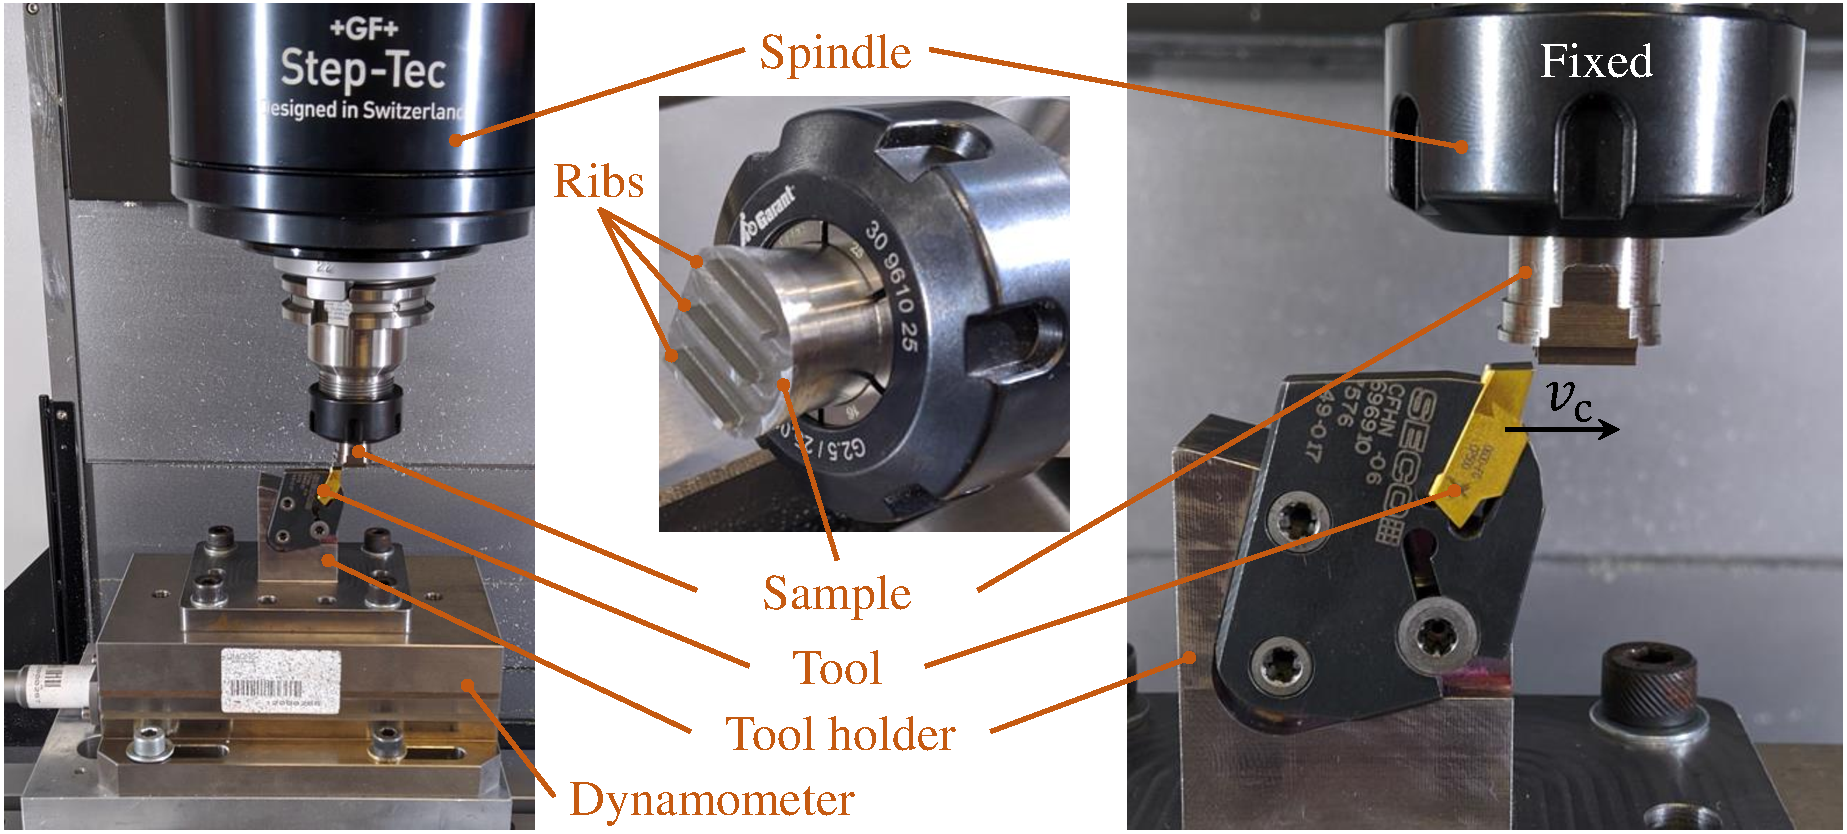
\includegraphics[width = 140 mm]{Figures/ExpSetup} % 140 mm, 1.5\columnwidth
\caption{Experimental setup}
\label{fig:ExpSetup}
\end{figure}

%
\begin{table}[!h]
\begin{center}
\caption{\label{tab:CutCond} Cutting conditions of the study}
\begin{tabular}{ll}
\hline\noalign{\smallskip}
Parameter  & Values\\
\noalign{\smallskip}\hline\noalign{\smallskip}
Cutting speed, $v_c$ (\unit{\metre\per\min}) & 5, 7.5, 10, 20, 30, 40\\
Uncut chip thickness, $h$ (\unit{\um}) & 40, 60, 80\\
Cutting edge inclination, $\lambda_s$ (\unit{\degree}) & 0, 6\\
Width of the workpiece (\unit{\mm}) & 1\\
Length of the workpiece (\unit{\mm}) & 10\\
Width of the cutting edge (\unit{\mm}) & 6 (1.1 in the model)\\
Cutting edge radius, $r_\beta$ (\unit{\um}) & 20\\
Rake angle, $\gamma_0$ (\unit{\degree}) & 15\\
Clearance angle, $\alpha_0$ (\unit{\degree}) & 2\\
\noalign{\smallskip}\hline
\end{tabular}
\end{center}
\end{table}
%

Forces are measured with a 3-component Kistler 9257B dynamometer and are amplified by a Kistler 5070A charge amplifier. Acquisition is performed at \qty{3}{\kHz} using a Kistler 5697A2 data acquisition system and DynoWare software. The recorded forces are then filtered with a second-order low-pass Bessel filter at \qty{750}{\Hz} before calculating the average value of the steady state signal.

All chips are collected and observed with a Dino Lite digital microscope AM7013MZT (5~MP, magnification $20\times$ -- $250\times$). Each chip is measured 3 times along its length in order to obtain an average value representative of the whole chip.

%%%%%%%%%%%%%%%%%%%%%%%%%%
\section{Finite element model}
\label{FEM}
%%%%%%%%%%%%%%%%%%%%%%%%%%

\subsection{Modelling choices}

The main objectives of a predictive model are the accurate modelling of trends in results as conditions change and the good agreement of predicted values with experimental values (exact values are not expected due to experimental dispersions of at least \qty{10}{\%} around the mean values). This type of model is intended to support future choices and developments without the need for experimental data. No assumptions are made about the geometry of the workpiece in the model (i.e., its width is the same as in experiments), while keeping the calculation time relevant for industrial applications. The CEL formulation is adopted to model the dry orthogonal and free oblique cutting tests with Abaqus/Explicit 2020. The 3D model is composed of a fixed Lagrangian tool and a Eulerian part (Figure \ref{fig:BC}). Chip formation occurs by plastic flow through the Eulerian domain without mesh distortion. The Eulerian formulation allows for chip formation without damage properties, by removing modelling assumptions. These two features contribute to the cutting models providing accurate results and realistic chips \cite{ducobu_Application_2016}.

\begin{figure}[!h]
\centering
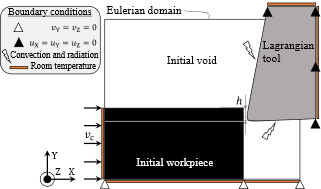
\includegraphics[width = 140 mm]{Figures/BC} % 90 mm, \columnwidth
\caption{Boundary conditions and schematic initial geometry of the model}
\label{fig:BC}
\end{figure}

As shown in Figure \ref{fig:FEConfig}, the full width of the workpiece (\qty{1}{\mm}), i.e., one rib in the experiments, is modelled. To allow for chip formation and lateral flow, the Eulerian domain is wider (it includes the volume in which the material can move). The volume above the initial part is also meshed with Eulerian elements for the same reasons. As in the experiments and to satisfy the assumption of an orthogonal and oblique free cut, the tool is wider than the workpiece (it is \qty{1.1}{\mm} in the model and \qty{6}{\mm} in the experiments). It is very important to note that the models are the same for both inclination angles: they differ only in the rotation of the tool by \qty{6}{\degree} around the Y axis as in the experiments (Figure \ref{fig:FEConfig}). This, together with the absence of assumptions when developing the models, contributes to make the models predictive: no input is changed when the cutting conditions are changed.

\begin{figure}[!h]
\centering
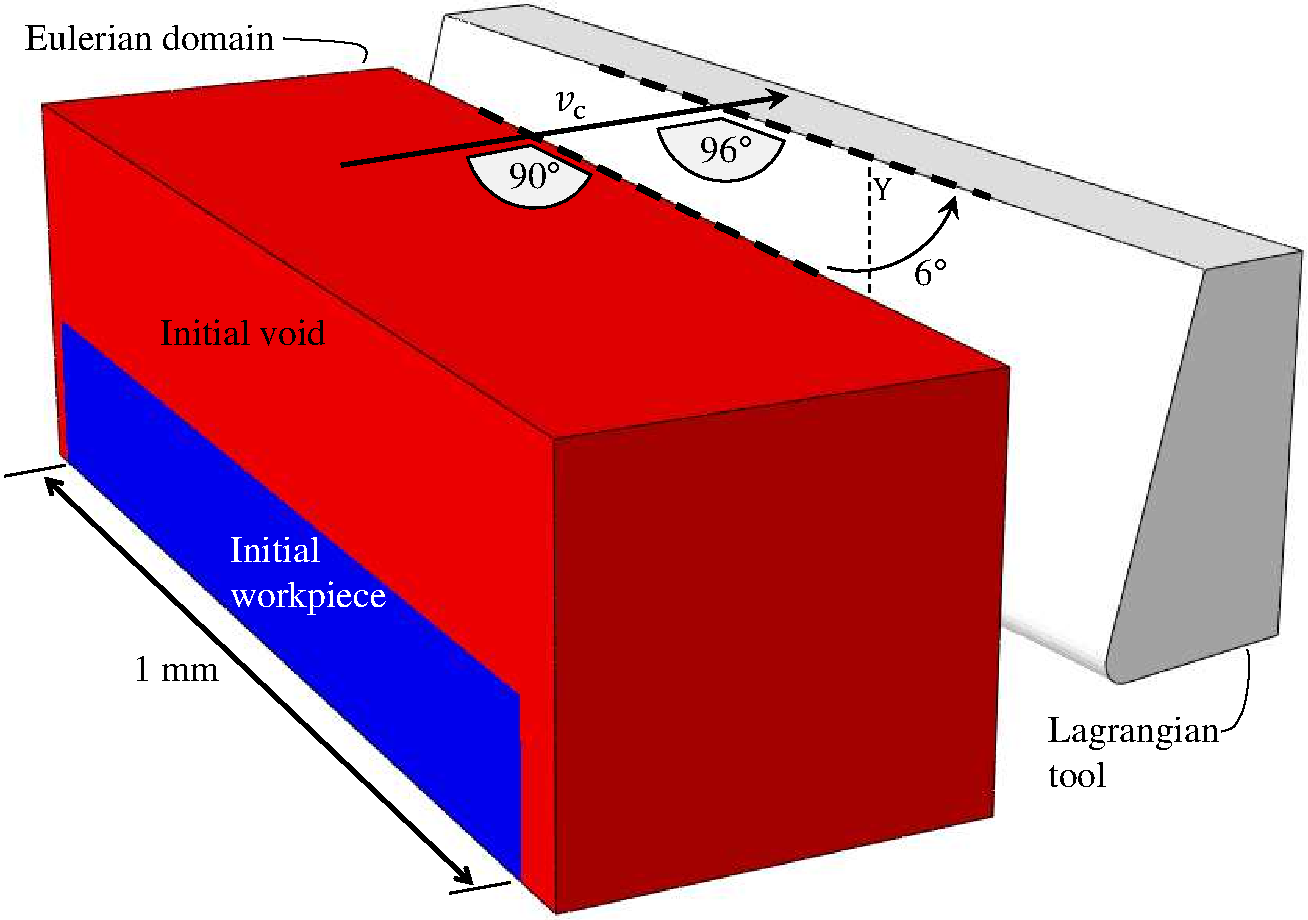
\includegraphics[width = 140 mm]{Figures/FEConfig}
\caption{Configuration of the FE model for $\lambda_s =$~\qty{6}{\degree}}
\label{fig:FEConfig}
\end{figure}

According to a previous sensitivity study of the mesh in orthogonal cutting with the CEL formulation \cite{ducobu_Finite_2017}, the edge size of the elements is \qty{5}{\um} in the plane parallel to the cutting speed. In the direction perpendicular to this plane, it is \qty{5}{\um} in the areas close to the lateral boundaries of the Eulerian domain and \qty{50}{\um} in the middle of the part. To reduce the computation time, the size of the model depends on the value of the uncut chip thickness. This results in a Eulerian domain (EC3D8RT 8-node 3D linear Eulerian elements, coupled mechanical-thermal behaviour and reduced integration) composed of \num{216550} to \num{273350} nodes and a Lagrangian domain (C3D8T 8-node 3D linear Lagrangian elements, coupled mechanical-thermal behaviour) of \num{4650} nodes.

The Ti6Al4V part is assumed to be thermo-elasto-viscoplastic (isotropic) and the inelastic thermal fraction is 0.9. The JC parameters set of Seo et al. \cite{seo_Constitutive_2005} is adopted because the value of $A$ corresponds to the value of the typical yield strength of Ti6Al4V and this set was found to provide the best results among the 20 sets available in the literature \cite{ducobu_Importance_2017}.  The TiN coated tungsten carbide (WC) tool is assumed to have linear elasticity. The material properties are given in Table \ref{tab:prop}.

%
\begin{table}[!h]
\begin{center}
\caption{\label{tab:prop} Materials properties \cite{seo_Constitutive_2005, _GRANTA_2020, milosevic_Thermophysical_2012}}
\begin{tabular}{lll}
\hline\noalign{\smallskip}
Young's modulus, $E$ (\unit{\GPa}) & Ti6Al4V & 113.8\textsuperscript{\textdagger}\\
 & WC & 650\\
Poisson's ratio, $\nu$ & Ti6Al4V & 0.34\\
 & WC & 0.2\\
Density, $\rho$ (\unit{\kg\per\cubic\m}) & Ti6Al4V & \num{4430}\\
 & WC & \num{14850}\\
Conductivity, $k$ (\unit{\W\per\metre\per\K}) & Ti6Al4V & 6.3\textsuperscript{\textdagger}\\
 & WC & 100\\
Expansion, $\alpha$ (\unit{\per\K}) & Ti6Al4V & \num{8.6e-6}\textsuperscript{\textdagger}\\
 & WC & \num{5e-6}\\
Specific heat, $c_{p}$ (\unit{\J\per\kg\per\K}) & Ti6Al4V & 531\textsuperscript{\textdagger}\\
 & WC & 202\\
\noalign{\smallskip}\hline\noalign{\smallskip}
JC flow stress & $A$ (\unit{\MPa}) & 997.9\\
 & $B$ (\unit{\MPa}) & 653.1\\
 & $C$ & \num{0.0198}\\
 & $m$ & 0.7\\
 & $n$ & 0.45\\
 & $\mdot{\varepsilon}_0$ (\unit{\per\s}) & 1\\
 & $T_{\text{room}}$ (\unit{\K}) & 293\\
 & $T_{\text{melt}}$ (\unit{\K}) & 1873\\
\noalign{\smallskip}\hline\noalign{\smallskip}
\end{tabular}
\end{center}
\vspace{-0.4cm}\textsuperscript{\textdagger}: Dependence on the temperature, value provided at \qty{293}{\K}
\end{table}
%

According to the experimental results of Rech et al. \cite{rech_Characterisation_2013}, it is assumed that Coulomb friction occurs at the tool-piece interface and that the coefficients of friction, $\mu$, and heat partition, $\beta$, depend on the cutting speed. The limiting shear stress, $\tau_{\text{max}}$, is included and is given by:
%
\begin{equation}
\tau_{\text{max}} = \frac{\text{yield stress}}{\sqrt{3}} = \frac{A}{\sqrt{3}}
\end{equation}
%
All the friction energy is converted into heat. Table \ref{tab:fricHeat} shows the friction coefficients adopted in this study.

\begin{table}[!h]
\begin{center}
\caption{\label{tab:fricHeat} Friction and heat transfer coefficients \cite{rech_Characterisation_2013, _GRANTA_2020}}
\begin{tabular}{lll}
\hline\noalign{\smallskip}
Cutting speed, $v_c$ (\unit{\m\per\min}) & $\mu$ & $\beta$\\
\noalign{\smallskip}\hline\noalign{\smallskip}
5 & 0.24 & 1\\
7.5 & 0.22 & 0.89\\
10 & 0.21 & 0.80\\
20 & 0.19 & 0.63\\
30 & 0.18 & 0.55\\
40 & 0.17 & 0.50\\
\noalign{\smallskip}\hline\noalign{\smallskip}
Limiting shear stress, $\tau_{\text{max}}$ (\unit{\MPa}) & 576\\
Convection, $U$ (\unit{\W\per\square\m\per\K}) & 50\\
Radiation, $\epsilon$ & 0.3\\
\noalign{\smallskip}\hline\noalign{\smallskip}
\end{tabular}
\end{center}
\end{table}
%

An ambient temperature of \qty{293}{\K} is imposed on the top and right surfaces of the tool and on the left and bottom surfaces of the workpiece (Figure \ref{fig:BC}). It is assumed that radiation and convection occur on the rake and clearance faces of the tool. The initial temperature of the tool and workpiece is set to the room temperature (\qty{293}{\K}). The heat transfer coefficients are provided in Table \ref{tab:fricHeat}.

\subsection{Material model of Ti6Al4V}

The material model of Ti6Al4V used in all the numerical simulations proposed in the section \ref{sec:ExpNumResults} is a thermo-elasto-viscoplastic law using a flow criterion based on an Artificial Neural Network (ANN) identified for the chosen material and implemented in the Abaqus/Explicit code via a Fortran subroutine VUHARD as proposed by Pantalé et al. in \cite{pantale_Efficient_2022}.
The principle of this approach consists in replacing the analytical formulation of the flow law, based on a Johnson-Cook or Zerilli-Armstrong type model, and allowing the calculation of the flow stress $\sigma^y$ as a function of the plastic strain $\varepsilon^p$, the plastic strain rate, $\mdot{\varepsilon}^p$, and the temperature $T$, by a multi-layer ANN serving as universal approximator. Thus, the parameters of the neural network can be directly identified from the experimental data without having to postulate a behavioural model, which simplifies the procedure and allows greater flexibility in the definition of the model.
The proposed approach also allows, as shown in Pantalé et al. \cite{pantale_Efficient_2022}, to compute the three derivatives of the flow stress $\sigma^y$ with respect to the three input variables of the model, a necessary step to implement this model as a flow law in the form of a VUHARD subroutine in the FEM code Abaqus/Explicit, using the exact same network architecture and identified trained parameters as the one used to compute the flow stress $\sigma^y$.

In order to verify the influence of the neural network complexity on the numerical results of the simulation and on the computation time, several ANN architectures are tested afterwards (in \ref{subsec:nberneu}). The chosen global architecture has 2 hidden layers with a variable number of neurons for the first hidden layer ($\zeta$~=~9 to 17) and 7 neurons for the second hidden layer, 3 inputs (the plastic strain, $\varepsilon^p$, the plastic strain rate, $\mdot{\varepsilon}^p$, and the temperature, $T$) and one output (the yield strength, $\sigma^y$). The global architecture of this type of ANN is given in Figure \ref{fig:ANN} for 9 neurons in the first hidden layer. According to Pantalé et al. \cite{pantale_Efficient_2022}, this ANN is referred to as ANN 3-9-7-1-sig, as it has 3 inputs, 9 neurons in the first hidden layer, 7 neurons in the second hidden layer, 1 output and a sigmoid activation function.

\begin{figure}[!h]
\centering
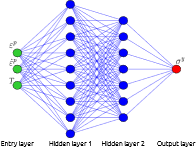
\includegraphics[width = 90 mm]{Figures/ANN}
\caption{Architecture of the ANN 3-9-7-1-sig used for the flow law}
\label{fig:ANN}
\end{figure}

In a preliminary phase, after having selected the global architecture of the neural network, it is necessary to proceed to its training from some inputs.
The inputs for this application were generated from the Johnson-Cook flow law expression reported in Equation (\ref{eq:J-C}) and the identified parameters reported in Table \ref{tab:prop}. This approach was chosen to demonstrate the ability of the neural network flow law to replace a classically formulated flow law such as Johnson-Cook's for the simulation of metal cutting. In future developments, experimental tests on a Gleeble thermomechanical simulator will be used to generate this network training data. The training data, presented in the form of a data table containing the plastic strain $\varepsilon^p$, the plastic strain rate $\mdot{\varepsilon}^p$, the temperature $T$ and the flow stress $\sigma^y$, is processed by a learning algorithm, developed at LGP, in Python, using the Tensorflow library. One hour of training on a Dell XPS13 7390 laptop running Ubuntu 20.04 64~bits with 16~GiB of Ram and an Intel 4-core i7-10510U processor allow obtaining the converged parameters of the ANN model.

Once this learning phase is completed, the neural network parameters resulting from the learning process are used directly by a Python program, in charge of automatically generating the Fortran source code of the VUHARD subroutine in order to compute the flow stress $\sigma^y$ and its three derivatives, required for the explicit Abaqus FEM code.

The main advantage of this approach (the use of an ANN), after the learning phase, is that, for example, the output $\sigma^y$ of the network is now linked to the inputs $\varepsilon^p$, $\mdot{\varepsilon}^p$, and $T$ by the equations (\ref{eq:ANN-preprocess}) to (\ref{eq:ANN-vonMises}) for a two hidden layers neural network with a sigmoid activation function as proposed previously.

Thus, in the VUHARD subroutine, the computation of the flow stress $\sigma^y$ from the 3 input variables $\varepsilon^p$, $\mdot{\varepsilon}^p$, and $T$ is performed using the following procedure. The first step is to scale the input data to the interval $[0,1]$ using the following equation:

\begin{equation}
\overrightarrow{x} =
\begin{cases}
x_1 = \frac{\varepsilon^p - [\varepsilon^p]_{min}}{[\varepsilon^p]_{max} - [\varepsilon^p]_{min}}\\
x_2 = \frac{\ln(\mdot{\varepsilon}^p)-[\ln(\mdot{\varepsilon}^p)]_{min}}{[\ln(\mdot{\varepsilon}^p)]_{max}-[\ln(\mdot{\varepsilon}^p)]_{min}}\label{eq:ANN-preprocess}\\
x_3 = \frac{T-[T]_{min}}{[T]_{max}-[T]_{min}}
\end{cases}
\end{equation}
where quantities $[\ ]_{min}$ and $[\ ]_{max}$  are the boundaries of the range of the corresponding field during the training phase. Corresponding values, for the proposed case, are given in \ref{sec:appendix-1}.
According to the architecture of the network, the outputs of the neurons of the first hidden layer $\overrightarrow{y_1}$ are given by the following equation:
\begin{equation}
\overrightarrow{y_1} = \sigmoid\left(\w_1 \dotp \overrightarrow{x}+ \overrightarrow{b_1}\right)\label{eq:ANN-y1}
\end{equation}
where, $\w_1$ and $\overrightarrow{b_1}$ are the weights and biases associated with the first hidden layer and $\sigmoid()$ is the sigmoid activation function defined by the equation (\ref{eq:sigmoid}) :
\begin{equation}
\sigmoid(x)=\frac{1}{1 + \e{-x}}\label{eq:sigmoid}
\end{equation}

Then, the output of the neurons of the second hidden layer is given by the equation (\ref{eq:ANN-y2}) :
\begin{equation}
\overrightarrow{y_2} = \sigmoid\left(\w_2 \dotp \overrightarrow{y_1}+ \overrightarrow{b_2}\right)\label{eq:ANN-y2}
\end{equation}
where, $\w_2$ and $\overrightarrow{b_2}$ are the weights and biases associated with the second hidden layer.
Finally, the $\sigma^y$ output of the ANN is thus given by the equation (\ref{eq:ANN-vonMises}) :
\begin{equation}
\sigma^y =  \left([\sigma^y]_{max}-[\sigma^y]_{min}\right) \left(\overrightarrow{w}^T \dotp \overrightarrow{y_2} + b\right) + [\sigma^y]_{min} \label{eq:ANN-vonMises}
\end{equation}
where, $\overrightarrow{w}$ and $b$ are the weights and the bias associated with the output layer. 

On the other hand, the three derivatives of the yield stress $\sigma^y$ with respect to the three input variables $\varepsilon^p$, $\mdot{\varepsilon}^p$, and $T$ are given by the equation (\ref{eq:derivatives-ANN}):
\begin{equation}
\begin{cases}
\partial \sigma^y/\partial \varepsilon^p = s'_1 \frac{[\sigma^y]_{max} -[\sigma^y]_{min}}{[\varepsilon^p]_{max} -[\varepsilon^p]_{min}}\\
\partial \sigma^y/\partial\mdot{\varepsilon}^p = s'_2 \frac{[\sigma^y]_{max} -[\sigma^y]_{min}}{\left[[\mdot{\varepsilon}^p]_{max} -[\mdot{\varepsilon}^p]_{min}\right]\mdot{\varepsilon}^p}\\
\partial \sigma^y/\partial T = s'_3 \frac{[\sigma^y]_{max} -[\sigma^y]_{min}}{[T]_{max} -[T]_{min}}
\end{cases}\label{eq:derivatives-ANN}
\end{equation}

where $s'_i$ is the $i^{th}$ component of the vector $\overrightarrow{s}'$ defined by the equation (\ref{eq:der-2-sig}):
\begin{equation}
\overrightarrow{s}' =\w_1^T \dotp \left[\w_2^T \dotp \left( 
\frac{\overrightarrow{w} \ccirc \e{-\overrightarrow{y_2}}}
{\left[1 + \e{-\overrightarrow{y_2}}\right]^2}\right)\ccirc \left(\frac{
\e{-\overrightarrow{y_1}}}
{\left[1 + \e{-\overrightarrow{y_1}}\right]^2}
\right)\right]\label{eq:der-2-sig}
\end{equation}
and $\ccirc$ is the elements-wise product, known as the Hadamard product.
In equations (\ref{eq:ANN-preprocess}) to (\ref{eq:der-2-sig}), quantities $\w_1$, $\w_2$, $\overrightarrow{w}$, $\overrightarrow{b_1}$, $\overrightarrow{b_2}$ and $b$ are evaluated by the training procedure of the ANN. Corresponding values for an ANN containing 9 neurons in the first hidden layer and 7 neurons in the second hidden layer are reported in \ref{sec:appendix-1}.
The set of equations (\ref{eq:ANN-preprocess}) to (\ref{eq:der-2-sig}), together with the network parameters identified in the learning phase, is automatically translated into a VUHARD Fortran subroutine used by the FEM code Abaqus to simulate the cutting model.

Because of the large number of identified parameters for all the ANN models (from 114 to 202 for 9 and 17 neurons for the first hidden layer, respectively), the other 4 sets of ANN parameters used in this publication can be found in \cite{pantale_Coefficients_2022}.

\subsection{Sensitivity study of the results to mass scaling}

FE modelling of the cutting process is very expensive in terms of CPU time due to the coupling of many nonlinear phenomena and the large amount of tiny finite elements. Mass scaling (MS) is introduced into the model to reduce the CPU computation time while checking that it does not influence the results (forces and energies) via a mass scaling sensitivity study. MS factors, $\dnsp{MS}{f}$, ranging from \num{1E6} (theoretical CPU time scale of $\sqrt{\dnsp{MS}{f}} = \num{1000}$) to 1 (no scale) were used for a cutting condition ($\lambda_s$~=~\qty{0}{\degree}, $v_c$~=~\qty{30}{\m\per\min} and $h$~=~\qty{60}{\um}). The same signal processing procedure is applied to the numerical forces as to the experimental forces (cf. \ref{ExpSet}): they are filtered with a second-order low-pass Bessel filter at \qty{750}{\Hz} before calculating the steady state average value. Table \ref{tab:MS} gives the results of the model with MS normalized ($\hat{F_i}$) by those of the model without MS:

\begin{equation}
\hat{F_i} = \frac{F_i\text{ with MS}}{F_i\text{ without MS}}
\end{equation}
%
with $i = c$ for the cutting force and $i = f$ for the feed force. As expected, the real speed-up does not increase linearly with the $\dnsp{MS}{f}$, but it remains significant. A $\dnsp{MS}{f}$ of \num{1E6} leads to an unstable computation and a $\dnsp{MS}{f}$ of \num{1E5} leads to erratic force evolutions. These results are confirmed by high values of the ratio of the kinetic ($KE$) to the internal ($IE$) energies (it should not exceed a few \unit{\%} \cite{wang_Investigation_2011, ducobu_Introduction_2015}). A value of $\dnsp{MS}{f}$ of 1E3 is chosen as it offers a good balance between reducing the computation time and the impact on the forces, while keeping the $\frac{KE}{IE}$ below \qty{1}{\%}. To provide an order of magnitude of CPU computation time, between \qty{10}{\hour} and \qty{50}{\hour} (depending on the value of $h$) are required on 4 cores of an Intel i7-5700HQ CPU at \qtyrange{2.7}{3.5}{\GHz}.
%
\begin{table}[!h]
\begin{center}
\caption{\label{tab:MS} MS sensitivity study (selected MS factor, $\dnsp{MS}{f}$, in bold, $\hat{\snsp{F}{c}}$: normalized cutting force, $\hat{\snsp{F}{f}}$: normalized feed force, $KE$: kinetic energy, $IE$: internal energy)}
\begin{tabular}{llllll}
\hline\noalign{\smallskip}
$\dnsp{MS}{f}$ & CPU scaling & Speed-up & $\hat{\snsp{F}{c}}$ & $\hat{\snsp{F}{f}}$ & $\frac{KE}{IE}$ (\unit{\%})\\
\noalign{\smallskip}\hline\noalign{\smallskip}
1 & 1 & 1 & 1 & 1 & \num{2.3E-4}\\
\num{1E2} & 10 & 9 & 1.006 & 0.982 & \num{2.2E-2}\\
\textbf{\num{1E3}} & \textbf{32} & \textbf{21} & \textbf{1.008} & \textbf{0.940} & \textbf{\num{2.2E-1}}\\
\num{1E4} & 100 & 61 & 1.012 & 0.921 & 2.4\\
\num{1E5} & 316 & 173 & Erratic & Erratic & 22\\
\num{1E6} & 1000 & 207 & Unstable & Unstable & 58\\
\noalign{\smallskip}\hline
\end{tabular}
\end{center}
\end{table}
%

\subsection{Sensitivity study of the results to the number of neurons}
\label{subsec:nberneu}

The number of neurons in the hidden layers may influence the results. A sensitivity study on the number of neurons of the first hidden layer, $\zeta$, is performed in order to select the ANN offering the best balance between CPU computation time and quality of the results. The results of the study are provided in Table \ref{tab:NbNeurons}. $\check{F_i}$ corresponds to the results of the model with ANN normalized by those of the model with the built-in JC model:

\begin{equation}
\check{F_i} = \frac{F_i\text{ with ANN}}{F_i\text{ with JC}}
\end{equation}
%
They show no influence on the numerical results for the forces compared to the built-in Johnson-Cook model, only the computation time is influenced by the number of neurons in the first hidden layer and increases with it. This increase in computation time is not only due to the increasing complexity of the neural network with the number of neurons, but also to the need to go through a VUHARD user subroutine. A first hidden layer of 9 neurons is therefore selected as it leads to the smallest increase in CPU computation time, without influence on the final result.

%
\begin{table}[!h]
\begin{center}
\caption{\label{tab:NbNeurons} Sensitivity of the forces to the number of neurons of the first layer, $\zeta$
(selection in bold, $\check{\snsp{F}{c}}$: normalized cutting force, $\check{\snsp{F}{f}}$: normalized feed force)}
\begin{tabular}{llll}
\hline\noalign{\smallskip}
$\zeta$  & Time increase (\unit{\%}) & $\check{\snsp{F}{c}}$ & $\check{\snsp{F}{f}}$\\
\noalign{\smallskip}\hline\noalign{\smallskip}
Built-in & 0 & 1.000 & 1.000\\
\textbf{9} & \textbf{6} & \textbf{1.000} & \textbf{0.999}\\
11 & 6 & 1.001 & 1.000\\
13 & 7 & 1.000 & 0.998\\
15 & 8 & 1.001 & 1.001\\
17 & 10 & 1.000 & 1.000\\
\noalign{\smallskip}\hline
\end{tabular}
\end{center}
\end{table}
%

%%%%%%%%%%%%%%%%%%%%%%%%%%
\section{Experimental and numerical results\label{sec:ExpNumResults}}
\label{Results}
%%%%%%%%%%%%%%%%%%%%%%%%%%

An example of the temporal evolution of the numerical and experimental forces is plotted for the 3 directions in Figure \ref{fig:ExpNum_Forces_v10_40µ_6} at $\lambda_s =$~\qty{6}{\degree}, $v_c =$~\qty{10}{\m\per\min} and $h =$~\qty{40}{\m\per\min}. The FE models are calculated up to a few microseconds after the stationary state is reached. Then, a linear extrapolation (dashed line between the last two markers in Figure \ref{fig:ExpNum_Forces_v10_40µ_6}) is used to provide numerical values for the same time range as the experimental values. The average and standard deviation ($2\,\sigma$) are calculated from the 3 experimental values. The resulting dispersion is shown in Figure \ref{fig:ExpNum_Forces_v10_40µ_6} around the average values of each force. Steady state takes longer to be reached for the experiments than for the numerical model, in particular for the cutting force. The dispersion around the evolution of the average force is greater for the feed force than for the cutting force, while the average value of the feed force is \qty{46}{\%} of the average value of the cutting force. The numerical cutting force is very close to the experimental average cutting force; it is only \qty{4}{\%} higher. This difference, $\Delta j$, is calculated by :

%
\begin{equation}\label{eq:diff}
\Delta j = \frac{\left|j^\text{(sim)} - j^\text{(exp)}\right|}{j^\text{(exp)}}\times 100
\end{equation}
%
where $j$ is the cutting force, the feed force, the passive force or the chip thickness. $j^\text{(sim)}$ is the average value from the simulation, while $j^\text{(exp)}$ is the average experimental value.

The numerical feed force is underestimated by the model, but is within the \qty{95}{\%} experimental confidence interval. The numerical passive force difference is also underestimated and is not within the narrower experimental dispersion. The difference between the average values of the experimental and numerical feed and passive forces is \qty{25}{\%}. A less well modelled feed force than the cutting force is typical of FE models of the cutting process and the difference with the experimental value is similar to other studies for a narrower range of cutting conditions \cite{sima_Modified_2010, ducobu_Material_2016, karpat_Temperature_2011, zhang_Chip_2011,afrasiabi_NumericalExperimental_2021}. Hardt and Bergs \cite{hardt_Three_2021} also obtained larger differences for feed and passive force than for cutting force. The difference for passive force was higher than for feed force, which is the opposite observation of this work.

\begin{figure}[!h]
\centering
\includegraphics[width = 140 mm]{Figures/ExpNum_Forces_v10_40µ_6}
\caption{Temporal evolutions of experimental (E) and numerical (N) forces at $\lambda_s =$~\qty{6}{\degree}, $v_c =$~\qty{10}{\m\per\min} and $h =$~\qty{40}{\um} with dispersion around average experimental values (linear extrapolation of numerical values in dashed)}
\label{fig:ExpNum_Forces_v10_40µ_6}
\end{figure}

Numerical chips at $v_c =$~\qty{10}{\m\per\min} and $h =$~\qty{40}{\um} for $\lambda_s =$~\qty{0}{\degree} and $\lambda_s =$~\qty{6}{\degree} are provided in Figures \ref{fig:ChipsNum} and \ref{fig:ChipsNumBack}. When the inclination of the cutting edge is \qty{0}{\degree}, both sides of the chip are identical and a symmetry plane can be drawn in the middle of the workpiece (Figure \ref{fig:ChipsNumBack} (a)). On the other hand, for an inclination of the cutting edge of \qty{6}{\degree}, the chip is no longer aligned with the workpiece. The chip bends to one side due to the orientation of the tool and symmetry is lost in both the geometry and the thermal and mechanical fields, as shown in figure \ref{fig:ChipsNumBack} (b). This produces helical chips for the inclination angle of \qty{6}{\degree} as in the experiments. Figure \ref{fig:ChipNumTop} shows the variation of the chip thickness across its width: it is thicker in the middle (i.e., the body of the chip) than on its sides. This underlines the importance of 3D modelling, even for the orthogonal cutting configuration as highlighted earlier \cite{ducobu_Finite_2017}. The 3D modelling also allows reproducing the lateral flow that occurs in the experiments for both values of cutting edge inclination (Figure \ref{fig:ChipsNum}), unlike a 2D model \cite{xu_Simulation_2021, ambrosio_New_2022, ducobu_Finite_2017}. Although this leads to higher computation times, future cutting models should be in 3D, even when orthogonal cutting is considered. In this case, it is recommended to take advantage of the symmetry of the configuration to reduce the computation time. This simplification has not been included in this study to avoid any difference in the FE models between the 2 inclinations of the cutting edge.

\begin{figure}[!h]
\centering
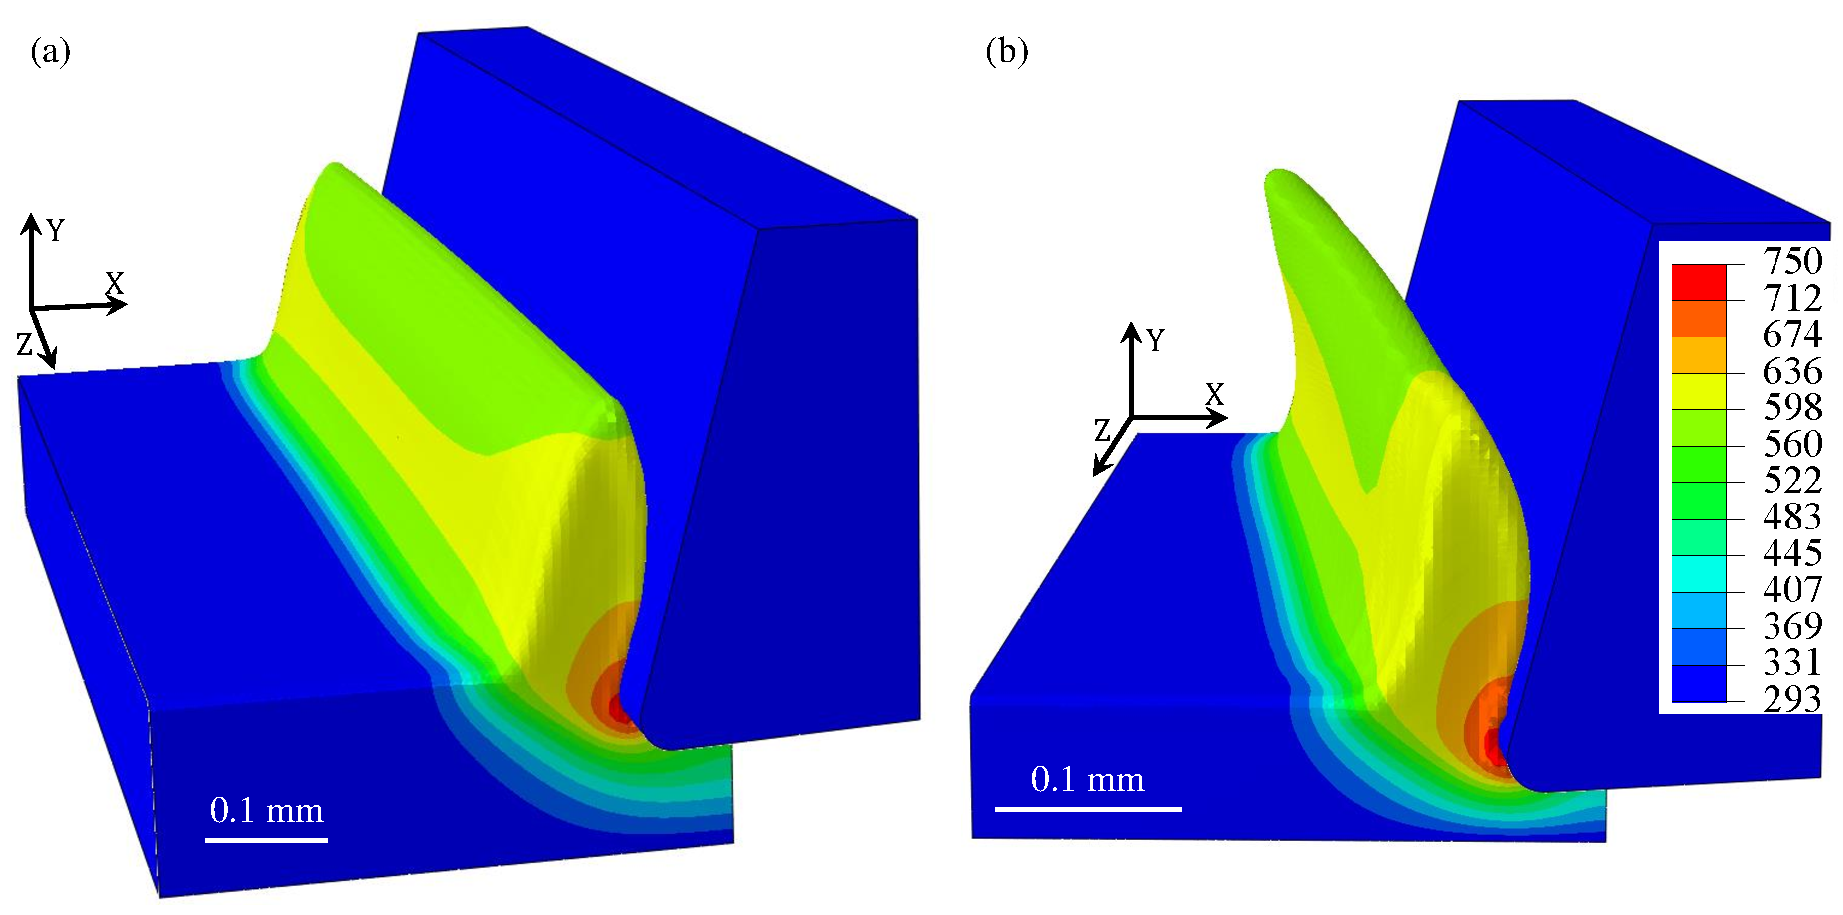
\includegraphics[width = 140 mm]{Figures/ChipsNum}
\caption{Temperature contours (in \unit{\K}) of the numerical chip after \qty{1.5}{\ms} at $v_c =$~\qty{10}{\m\per\min}, $h =$~\qty{40}{\um} and (a) $\lambda_s =$~\qty{0}{\degree}, (b) $\lambda_s =$~\qty{6}{\degree}}
\label{fig:ChipsNum}
\end{figure}

\begin{figure}[!h]
\centering
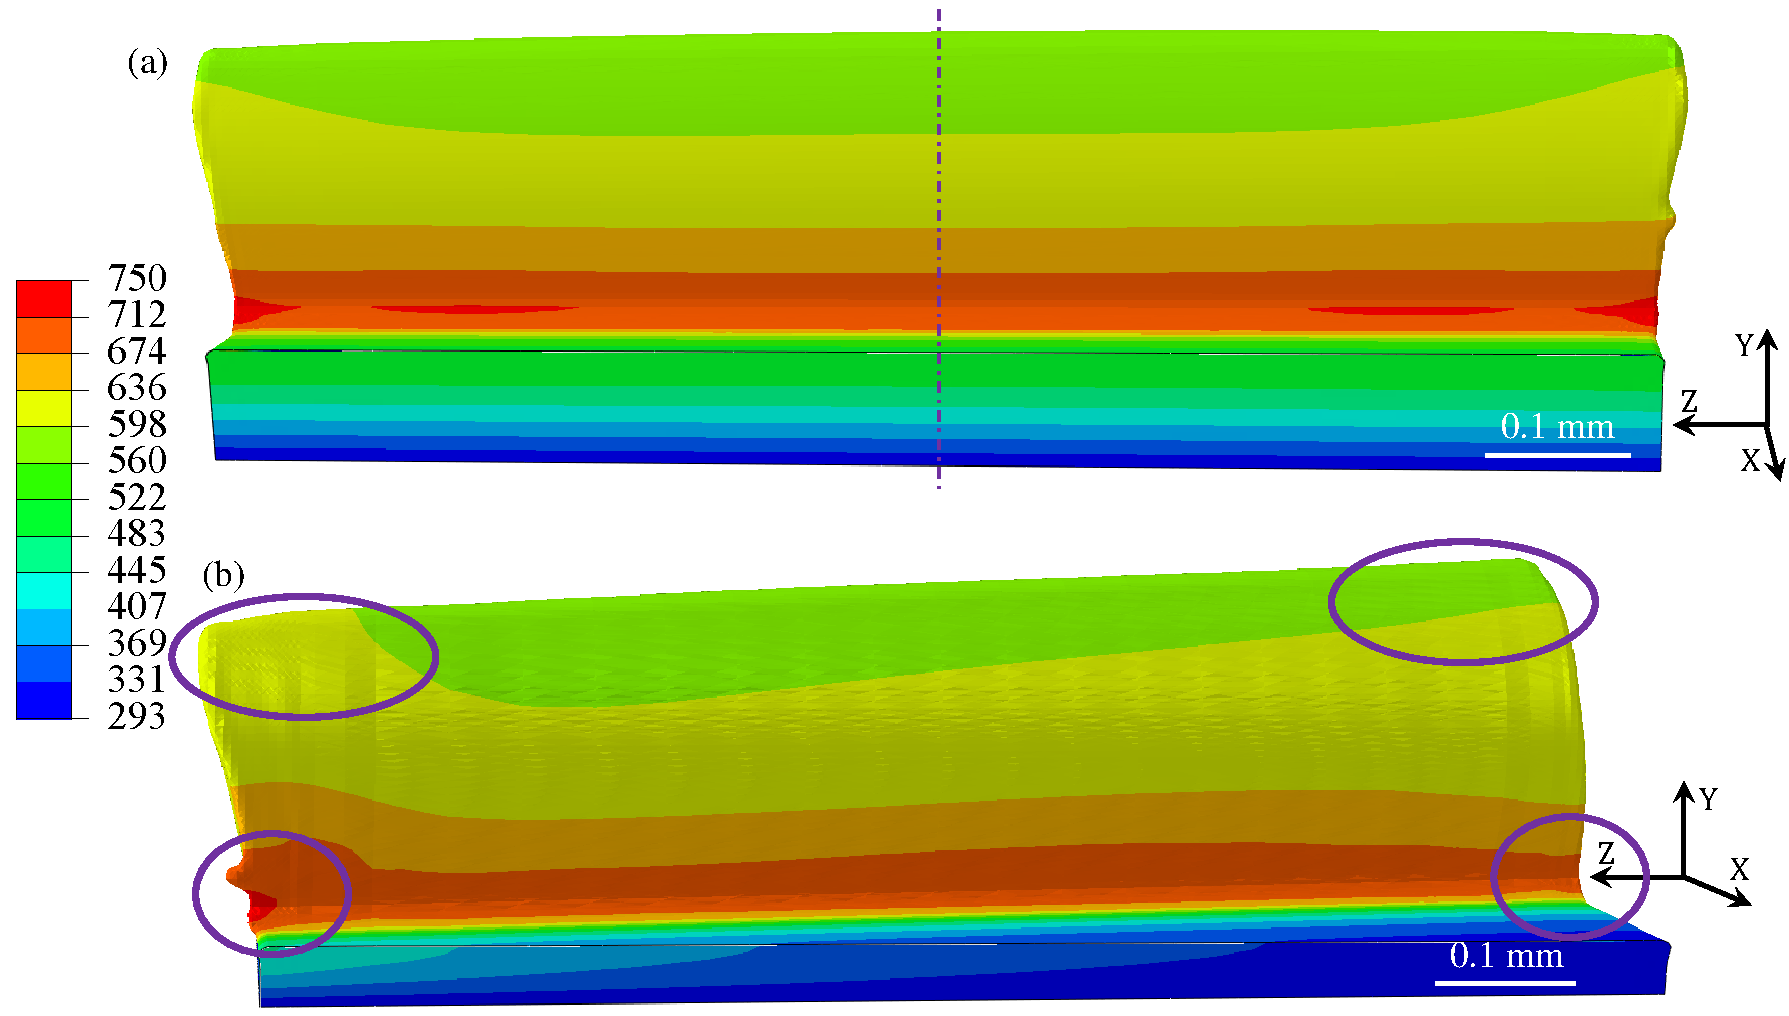
\includegraphics[width = 140 mm]{Figures/ChipsNumBack}
\caption{Temperature contours (in \unit{\K}) of the back of the numerical chip (tool is removed) after \qty{1.5}{\ms} at $v_c =$~\qty{10}{\m\per\min}, $h =$~\qty{40}{\um} and (a) $\lambda_s =$~\qty{0}{\degree}, (b) $\lambda_s =$~\qty{6}{\degree}}
\label{fig:ChipsNumBack}
\end{figure}

\begin{figure}[!h]
\centering
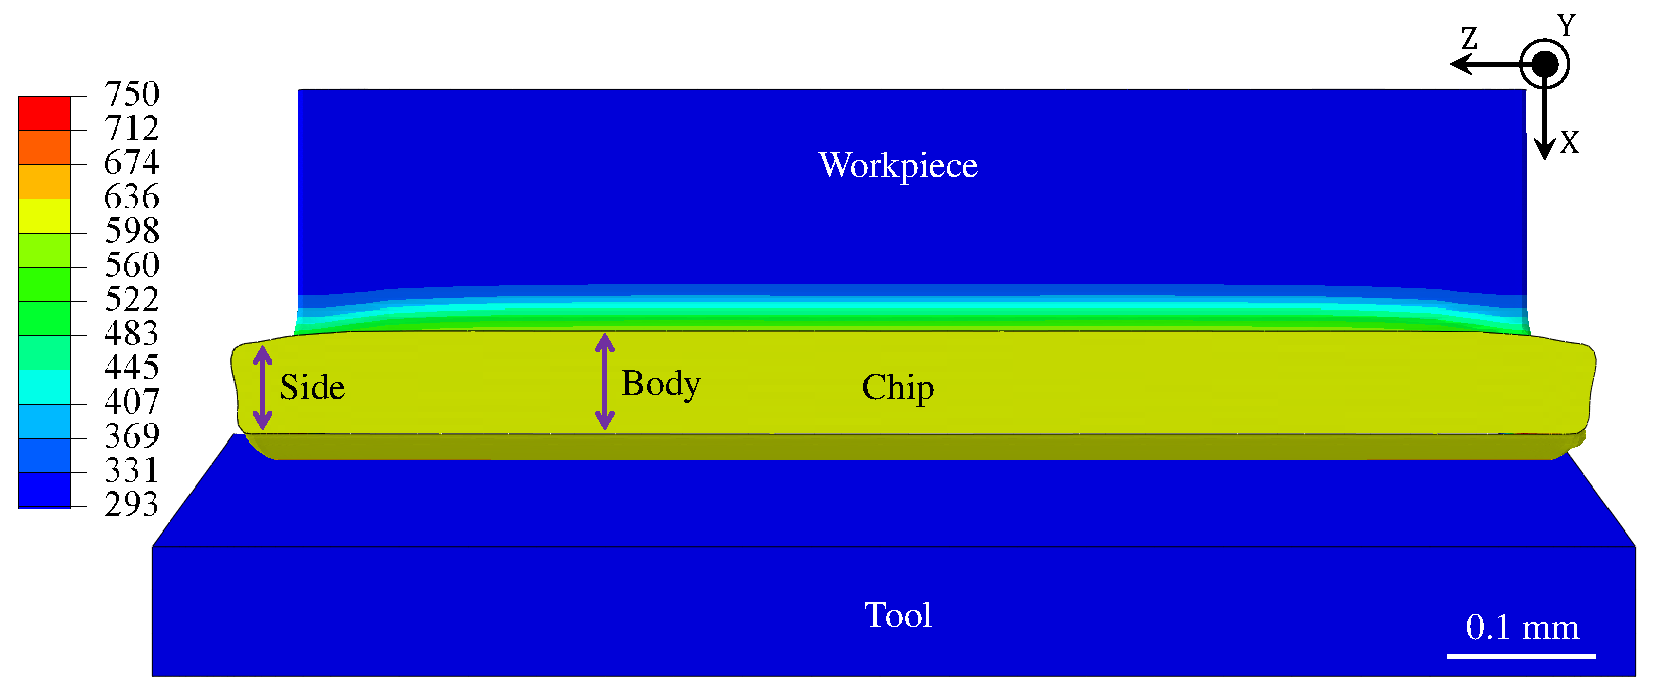
\includegraphics[width = 140 mm]{Figures/ChipNumTop}
\caption{Temperature contours (in \unit{\K}) of the top of the numerical chip after \qty{1.5}{\ms} at $v_c =$~\qty{10}{\m\per\min}, $h =$~\qty{40}{\um} and $\lambda_s =$~\qty{0}{\degree}}
\label{fig:ChipNumTop}
\end{figure}

Average values of the experimental forces and their dispersion are shown in Figures \ref{fig:Fx_0} to \ref{fig:Fz_6} together with the average numerical values. Passive force values are of course only plotted for $\lambda_s =$~\qty{6}{\degree} as they are equal to zero when $\lambda_s =$~\qty{0}{\degree}.

\begin{figure}[!h]
\centering
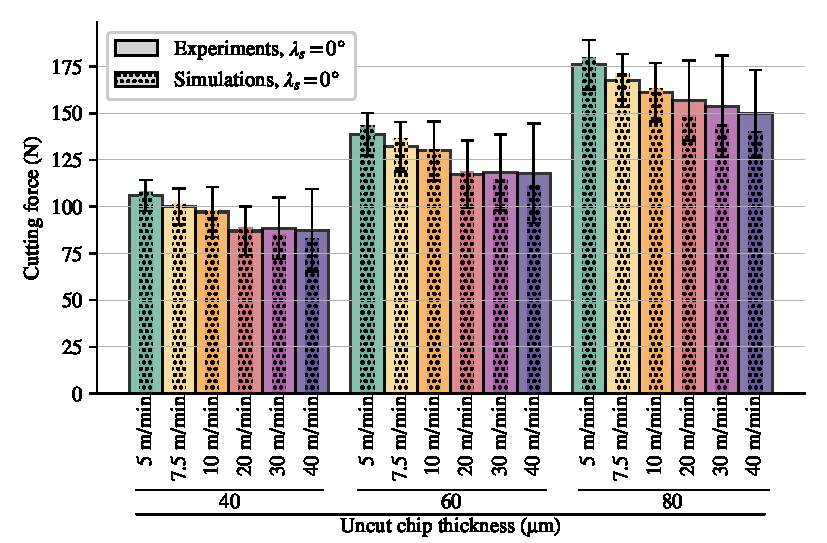
\includegraphics[width = 140 mm]{Figures/Fx_0}
\caption{Comparison of experimental and numerical cutting forces at the cutting edge inclination of \qty{0}{\degree} for the 3 uncut chip thicknesses and the 6 cutting speeds}
\label{fig:Fx_0}
\end{figure}

\begin{figure}[!h]
\centering
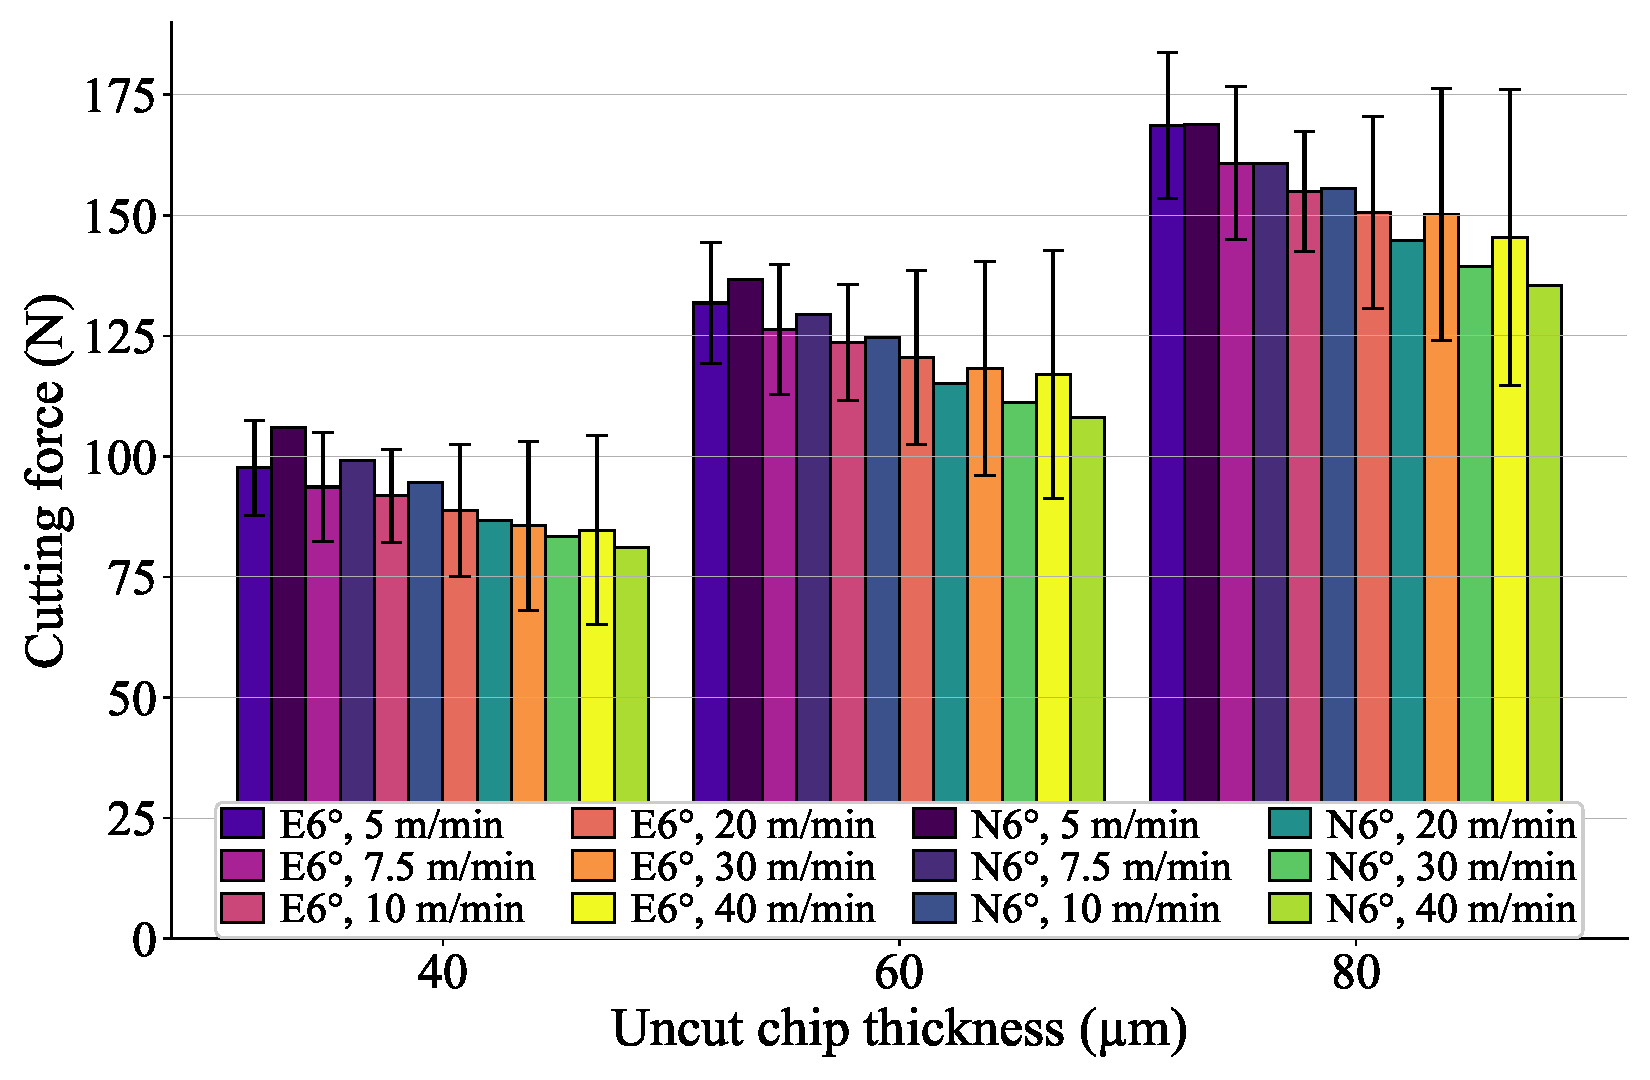
\includegraphics[width = 140 mm]{Figures/Fx_6}
\caption{Comparison of experimental and numerical cutting forces at the cutting edge inclination of \qty{6}{\degree} for the 3 uncut chip thicknesses and the 6 cutting speeds}
\label{fig:Fx_6}
\end{figure}

\begin{figure}[!h]
\centering
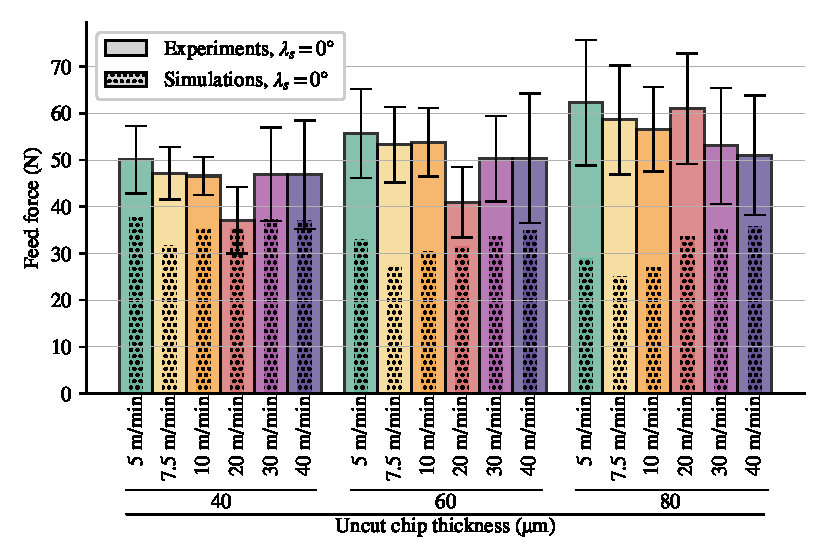
\includegraphics[width = 140 mm]{Figures/Fy_0}
\caption{Comparison of experimental and numerical feed forces at the cutting edge inclination of \qty{0}{\degree} for the 3 uncut chip thicknesses and the 6 cutting speeds}
\label{fig:Fy_0}
\end{figure}

\begin{figure}[!h]
\centering
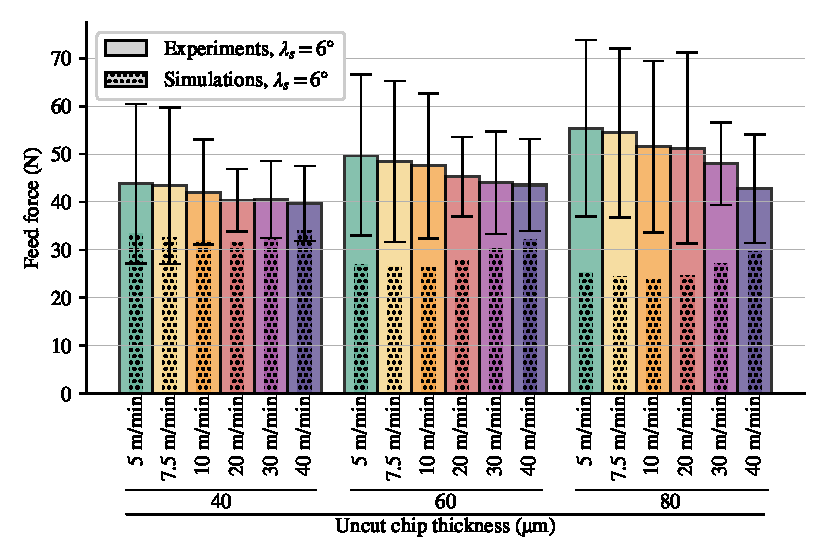
\includegraphics[width = 140 mm]{Figures/Fy_6}
\caption{Comparison of experimental and numerical feed forces at the cutting edge inclination of \qty{6}{\degree} for the 3 uncut chip thicknesses and the 6 cutting speeds}
\label{fig:Fy_6}
\end{figure}

\begin{figure}[!h]
\centering
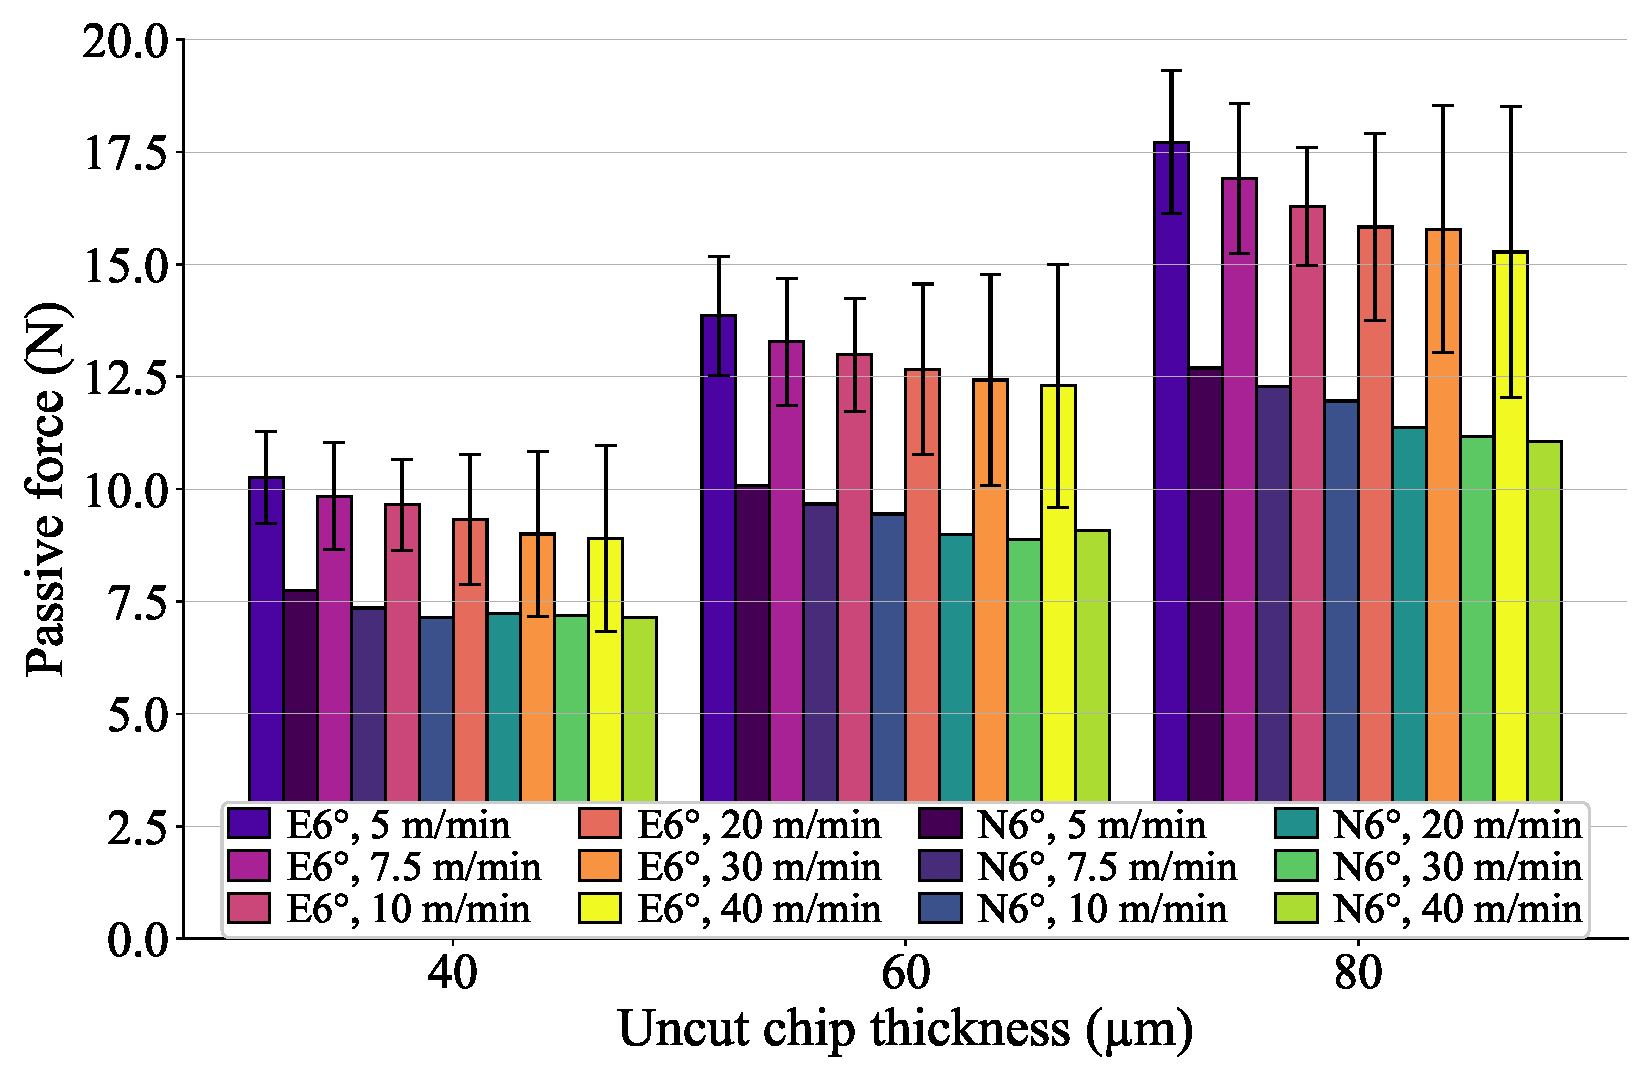
\includegraphics[width = 140 mm]{Figures/Fz_6}
\caption{Comparison of experimental and numerical passive forces at the cutting edge inclination of \qty{6}{\degree} for the 3 uncut chip thicknesses and the 6 cutting speeds}
\label{fig:Fz_6}
\end{figure}

The increase in cutting force with uncut chip thickness is clearly observed in Figures \ref{fig:Fx_0} and \ref{fig:Fx_6} for both experimental and numerical results at the 2 inclination angles, as well as the decrease in force with increasing cutting speed. This shows that temperature softening dominates strain rate hardening for Ti6Al4V and is accurately modelled. Increasing the inclination angle from \qty{0}{\degree} to \qty{6}{\degree} slightly reduces the cutting force; this is well captured by the model. For cutting speeds of \qtyrange{20}{40}{\m\per\min} and an inclination angle of \qty{0}{\degree}, $\snsp{F}{c}$ is almost constant with cutting speed for uncut chip thicknesses of \qty{40}{\um} and \qty{60}{\um}, while it decreases slightly for \qty{80}{\um}; this small stabilization is less marked for the model.

An increase in the deviation around the average value with the cutting speed is noted for values above \qty{10}{\m\per\min}. All numerical values are within \qty{95}{\%} confidence of the experiments (35 of the 36 conditions are within \qty{68}{\%} confidence). The average difference with the experiments is \qty{4}{\%}, which is remarkable, also considering the wide range of cutting conditions considered and the absence of model tuning. This underlines the predictive ability and accuracy of the FE model for both inclination angles.

Figures \ref{fig:Fy_0} and \ref{fig:Fy_6} show the results for the feed force, where the two clearest trends for the experiments are its decrease with the inclination angle and its increase with the uncut chip thickness (even though it is lower than expected). For \qty{80}{\um}, $\snsp{F}{f}$ decreases overall with $v_c$ in the experiments. For \qty{40}{\um} and \qty{60}{\um}, the force decreases at lower $v_c$, then increases for \qty{0}{\degree}, while a decrease is observed at all $v_c$ for \qty{6}{\degree} (the experimental dispersion is high for both inclination angles, but the average trend with cutting speed is clear at \qty{6}{\degree}, not at \qty{0}{\degree}). For the numerical values, the overall trend is the same for the 3 uncut chip thicknesses and the two inclination angles: a decrease for the lowest values of $v_c$ and then an increase. It should be noted that the numerical model does not correctly handle the trends of the feed forces: as Figure \ref{fig:Fy_6} clearly shows, the numerical forces have an overall increasing trend with the cutting speed, while their average value mainly decreases when the uncut chip thickness increases. The differences between the average numerical and experimental values increase with the uncut chip thickness: the forces are closer at \qty{40}{\um} than at \qty{80}{\um}. The numerical values are generally not within the \qty{95}{\%} confidence interval (they do not clearly change with the cutting conditions). Coupled with the differences in trends, this shows that $\snsp{F}{f}$ is less well modelled (the average difference is \qty{39}{\%}) than $\snsp{F}{c}$ as usual in FE modelling of the cutting process and even more so in 3D \cite{hardt_Three_2021}. The influence of the uncut chip thickness on the feed force should therefore be improved. The parameters of the material model are known to have an impact on the forces (and on the chip morphology) \cite{ducobu_Importance_2017,kugalurpalanisamy_Identification_2022}. The friction model should also be improved to strengthen the results \cite{hardt_Three_2021}.

The passive force is non-zero for the inclination angle of \qty{6}{\degree} (Figure \ref{fig:Fz_6}). Like the cutting force, it increases with the uncut chip thickness and decreases with the cutting speed. The comparison with experiments is broadly the same as for $\snsp{F}{c}$, except for a greater difference in the magnitude of $\snsp{F}{p}$ (the average difference is \qty{26}{\%}, but it is small in absolute terms -- less than \qty{5}{N}). Most of the numerical values do not fall within the experimental \qty{95}{\%} confidence interval. A lower magnitude of the passive force from the simulation than from the experiments with the correct trends when the cutting conditions change was also observed by Hardt and Bergs \cite{hardt_Three_2021}. The differences were mainly attributed to differences in cutting edge radius, friction modelling and material model. In this work, the impact of the cutting edge radius can be neglected as it is the same in the model as in the experiments.

As far as the chip morphology is concerned, all chips are continuous. For both the simulation and the experiments, the chip thickness ratio, $\lambda_h$ :
%
\begin{equation}
\lambda_h = \frac{h'}{h}
\end{equation}
%
with $h$ the uncut chip thickness and $h'$ the chip thickness, is almost independent of the uncut chip thickness (Figures \ref{fig:h0} and \ref{fig:h6}). It is slightly reduced from $\lambda_s =$~\qty{0}{\degree} to $\lambda_s =$~\qty{6}{\degree}, which means that the chip thickness decreases with the inclination angle. This influence is underestimated by the model: the reduction of $\lambda_h$ is smaller than in the experiments. The average difference between the experimental and numerical $\lambda_h$ is \qty{17}{\%} over the whole range of cutting conditions. The chip thickness ratio decreases with cutting speed due to the reduction in friction, which is correctly accounted for by the model. As with the feed force, the results should be improved by more complex friction models and a set of material parameters for which the identification includes forces and chip thickness: \cite{kugalurpalanisamy_Identification_2022}.

\begin{figure}[!h]
\centering
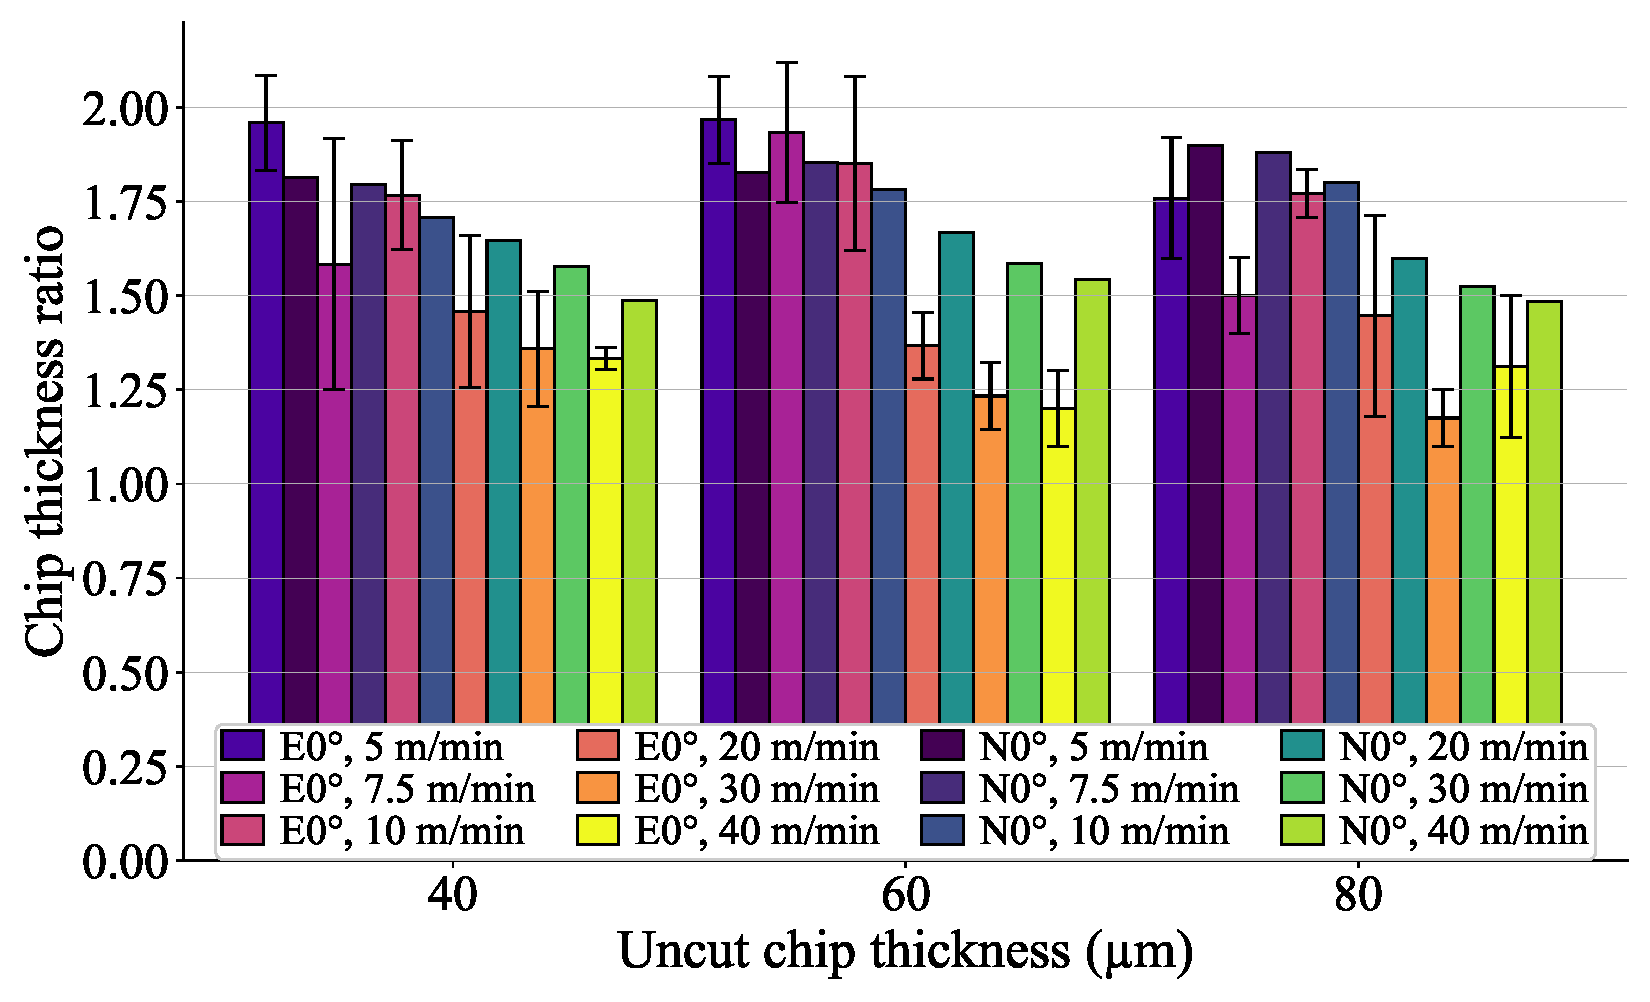
\includegraphics[width = 140 mm]{Figures/h0}
\caption{Comparison of experimental and numerical chip thickness ratios at the cutting edge inclination of \qty{0}{\degree} for the 3 uncut chip thicknesses and the 6 cutting speeds}
\label{fig:h0}
\end{figure}

\begin{figure}[!h]
\centering
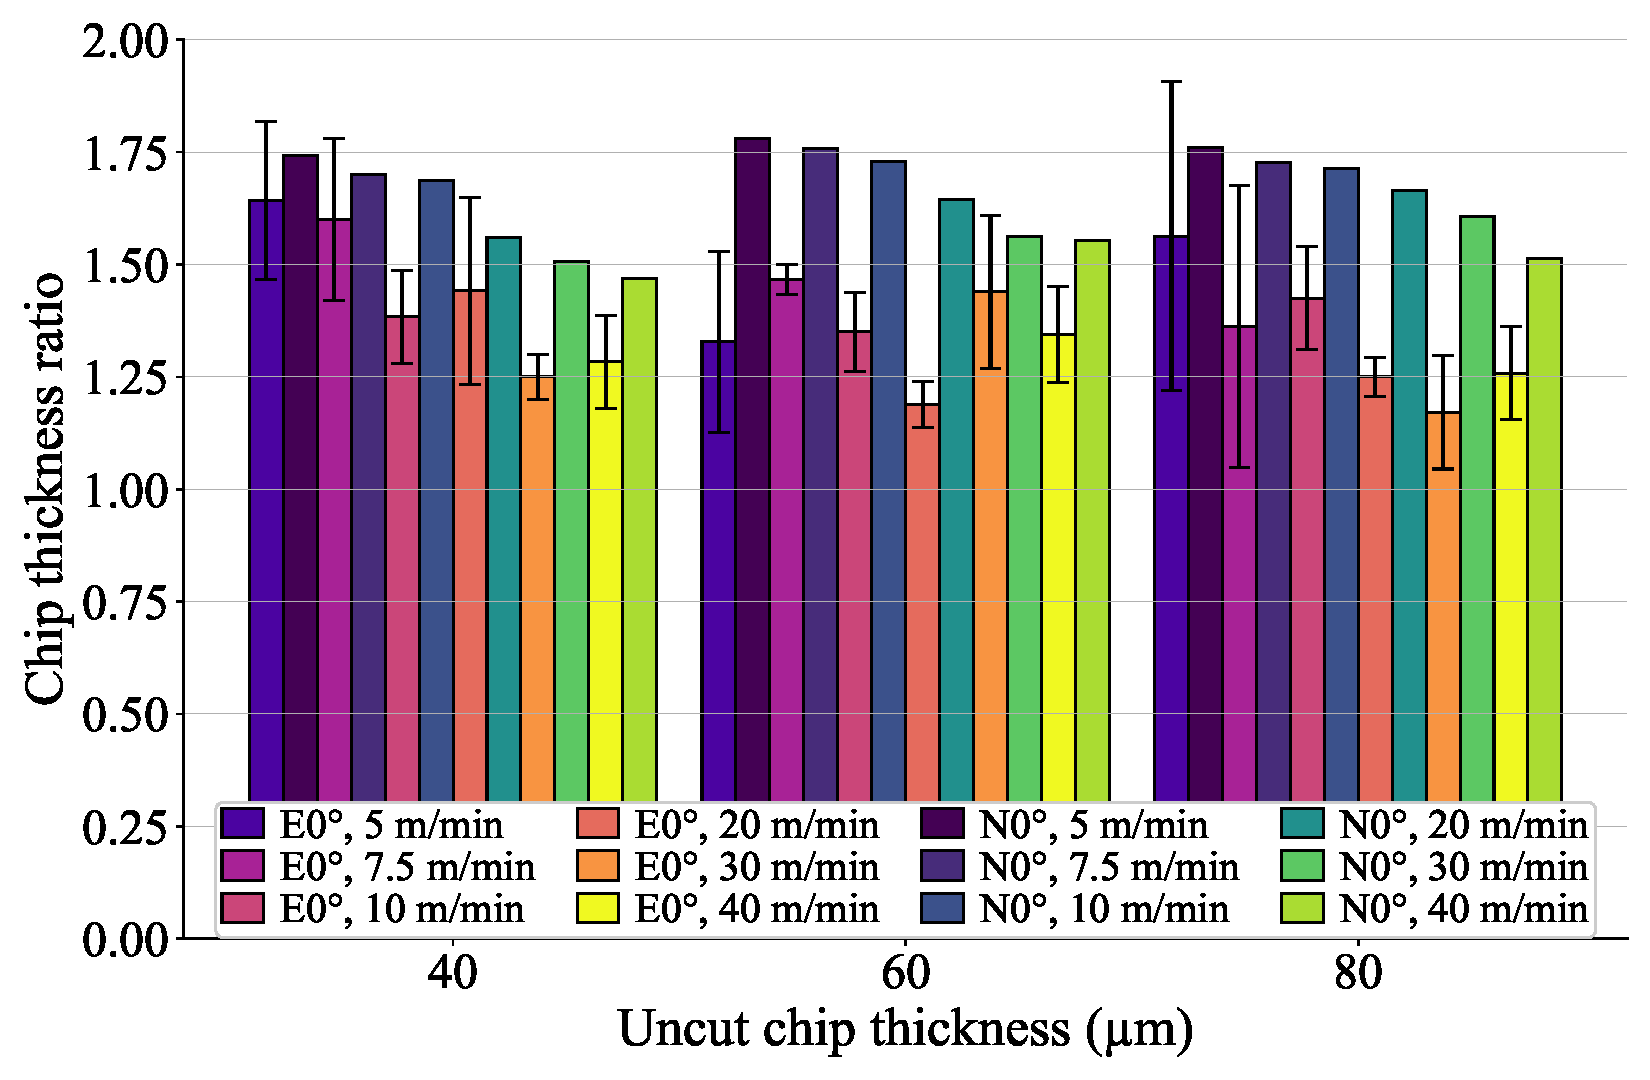
\includegraphics[width = 140 mm]{Figures/h6}
\caption{Comparison of experimental and numerical chip thickness ratios at the cutting edge inclination of \qty{6}{\degree} for the 3 uncut chip thicknesses and the 6 cutting speeds}
\label{fig:h6}
\end{figure}

The differences calculated according to the equation (\ref{eq:diff}) are presented in Table \ref{tab:Synth} to provide a quantitative overview of the results. The cutting force is the best modelled quantity as observed in the literature. This result was to be expected as the parameter set of the material model was selected mainly due to its good approximation of the cutting force \cite{ducobu_Importance_2017}. As this selection was made with a 2D model, the results show the ability of the model to correctly handle the third (passive) force. Based on the average differences, the performance of the model is very close for the cutting and feed forces for both cutting edge inclinations, although a small degradation (\qty{1}{\%} and \qty{2}{\%}, respectively) is noted for \qty{6}{\degree}. This degradation is more important (\qty{7}{\%}) for the chip thickness ratio and must be linked to the difference in passive force. Indeed, the chip thickness and out-of-plane force models are deeply linked. Improving the friction at the tool-workpiece interface should be a key point. It should be noted that the chip thickness is very well modelled under certain cutting conditions with a minimum difference of \qty{2}{\%}. The difference is larger for the feed force than for the passive force, a trend opposite to that of Hardt and Bergs \cite{hardt_Three_2021}. The average and range (min -- max) of the differences are larger for the feed force. The smaller range of the passive force confirms a shift for all cutting conditions, similar to the results of Hardt and Bergs \cite{hardt_Three_2021}. Again, the friction modelling should be the first aspect of the model to be improved in future developments.

%
\begin{table}[!h]
\begin{center}
\caption{\label{tab:Synth} Synthetic quantitative overview of the results: differences between the experimental and the numerical results (average difference for each cutting edge inclination, and maximal, minimal and average differences for all the conditions) for the cutting force, $\Delta \snsp{F}{c}$, the feed force, $\Delta \snsp{F}{f}$, the passive force, $\Delta \snsp{F}{p}$, and the chip thickness ratio, $\Delta \lambda_h$}
\begin{tabular}{lllll}
\hline\noalign{\smallskip}
Difference & $\Delta \snsp{F}{c}$ (\unit{\%}) & $\Delta \snsp{F}{f}$ (\unit{\%}) & $\Delta \snsp{F}{p}$ (\unit{\%}) & $\Delta \lambda_h$ (\unit{\%})\\
\hline\noalign{\smallskip}
Average $\lambda_s =$~\qty{0}{\degree} & 3 & 38 & -- & 14\\
Average $\lambda_s =$~\qty{6}{\degree} & 4 & 40 & 26 & 21\\
Max. global & 10 & 60 & 29 & 38\\
Min. global & 1 & 10 & 19 & 2\\
Average global & 4 & 39 & 26 & 17\\
\noalign{\smallskip}\hline\noalign{\smallskip}
\end{tabular}
\end{center}
\end{table}
%

%%%%%%%%%%%%%%%%%%%%%%%%%%
\section{Conclusions}
%%%%%%%%%%%%%%%%%%%%%%%%%%

An experimental and numerical study of the orthogonal and oblique free cutting of Ti6Al4V was carried out for a wide range of cutting conditions using an ANN-based flow law. The following main conclusions are drawn:
\begin{itemize}
  \item The experimental study was carried out with the same set-up in free orthogonal and free oblique cutting for the titanium alloy Ti6Al4V (the only change is the cutting edge inclination). This is a reference to evaluate the performance of the FE 3D model introducing an ANN-based flow law developed under the same conditions. An unpreviously seen wide range of cutting conditions, 36, is considered, including 2 cutting edge inclinations.
  \item A major novelty of this work is the accurate evaluation of the fundamental variables and their trends in 3D, without the need to adjust the numerical parameters and the model characteristics when the cutting conditions and the inclination angle are changed significantly. The mere fact of changing the inclination angle from free orthogonal cutting to oblique cutting while maintaining the quality of the results has no equivalent in the current literature, especially since no studies (experimental or numerical) on free oblique cutting are available.
  \item Taking into account the material's flow law by means of a neural network makes it possible to overcome the limitations of conventional flow laws and to reduce the approximations associated with the establishment of an analytical formulation of the flow law as conventionally adopted. The numerical model is then able to better reproduce the real behaviour of the material and to take into account thermomechanical transformations which are sources of non-linearities, difficult to take into account with an analytical flow law model. Current work, using a Gleeble thermomechanical simulator, on the behaviour of a modified carbon alloy AISI P20 shows the advantages of this approach compared to models in the literature such as Johnson-Cook, Zerilli-Armstrong \cite{gurusamy_Performance_2017} or Hansel-Spittel \cite{chadha_Approach_2018}, insofar as one is then able to better reproduce more complex material behaviours.
  \item The cutting force is the best modelled quantity with an average difference of \qty{4}{\%} with the experiments. Chip thickness ratio and passive force show a larger deviation from the experiments (\qty{17}{\%} and \qty{26}{\%}, respectively), but their trends as the cutting conditions change are accurate. This is in line with the expected results provided by a predictive model. The deviation for feed force is higher (\qty{39}{\%}), and opposite trends compared to the experimental reference are observed. The lack of influence of uncut chip thickness on friction in the model seems to be one of the aspects to be included as a priority in future work. The model is found to handle the occurrence of the third force, out of plane, well without significant degradation of the results.
  \item The predictive capabilities of the model make it suitable for the development of straight-edged tools, for example. This work also demonstrates the ability to model material behaviour with ANN and opens up possibilities in this promising direction.
\end{itemize}

%%%%%%%%%%%%%%%%%%%%%%%%%%
\section{Statements \& Declarations}
%%%%%%%%%%%%%%%%%%%%%%%%%%

\noindent\textbf{Funding}

\noindent The authors declare that this research received no external funding.\\

\noindent\textbf{Competing Interests}

\noindent The authors have no relevant financial or non-financial interests to disclose.\\

%\textbf{Availability of data and material}
%
%\textbf{Code availability}
%
%\textbf{Ethics approval and consent to participate}
%
%This article does not contain any studies with human participants or animals performed by any 
%authors.
%
%\textbf{Consent for publication}

\noindent\textbf{Author Contributions}

\noindent François Ducobu contributed to Data curation, Formal analysis, Investigation, Methodology, Software, Supervision, Validation, Visualization, Writing -- original draft and review \& editing (focussing on non ANN-related aspects). Olivier Pantalé contributed to Data curation, Formal analysis, Investigation, Methodology, Software, Validation, Visualization, Writing -- original draft and review \& editing (focussing on ANN-related aspects). Bert Lauwers contributed to Supervision and Writing -- review \& editing. All authors read and approved the final manuscript.

%%%%%%%%%%%%%%%%%%%%%%%%%%
%%% References
%%%%%%%%%%%%%%%%%%%%%%%%%%
%%%
%%% Following citation commands can be used in the body text:
%%% Usage of \cite is as follows:
%%%   \cite{key}          ==>>  [#]
%%%   \cite[chap. 2]{key} ==>>  [#, chap. 2]
%%%   \citet{key}         ==>>  Author [#]
%
%%% References with bibTeX database:
%
\bibliographystyle{model1-num-names}
\bibliography{Biblio}
%
%%% Authors are advised to submit their bibtex database files. They are
%%% requested to list a bibtex style file in the manuscript if they do
%%% not want to use model1-num-names.bst.
%
%%% References without bibTeX database:
%
%% \begin{thebibliography}{00}
%


%%% \bibitem must have the following form:
%%%   \bibitem{key}...
%%%
%
%% \bibitem{}
%
%% \end{thebibliography}
%


%%%%%%%%%%%%%%%%%%%%%%%%%%%
%%% The Appendices part is started with the command \appendix;
%%% appendix sections are then done as normal sections
\appendix
%
\section{Coefficients of the ANN 3-9-7-1-sig\label{sec:appendix-1}}

In this appendix, we present the values obtained after the training phase of an ANN containing 9 neurons in the first hidden layer and 7 neurons in the second hidden layer. Conforming to \cite{pantale_Efficient_2022}, this one is referred ANN-3-9-7-1-sig.
The training of the neural network was performed using a dataset containing \num{3430} data points defined by:
\begin{itemize}
\item \num{70} equidistant values for $\varepsilon^p\in[0,3]$, so that $[\varepsilon^p]_{min}=0$ and $[\varepsilon^p]_{max}=3$.
\item \num{7} plastic strain rates $\mdot{\varepsilon}^p\in[\qty{1}{\per\s}, \qty{10}{\per\s}, \qty{50}{\per\s}, \qty{500}{\per\s}, \qty{5000}{\per\s}, \qty{50000}{\per\s}, \qty{500000}{\per\s}]$, so that $[\ln(\mdot{\varepsilon}^p)]_{min}=0$ and $[\ln(\mdot{\varepsilon}^p)]_{max}=13.12236$.
\item \num{7} temperatures $T\in[\qty{293}{\K}, \qty{400}{\K}, \qty{500}{\K}, \qty{700}{\K}, \qty{900}{\K}, \qty{1200}{\K}, \qty{1500}{\K}]$, so that $[T]_{min}=\qty{293}{\K}$ and $[T]_{max}=\qty{1500}{\K}$.
\end{itemize}

Stresses in the training dataset ranges from $[\sigma^y]_{min}=\qty{171.4}{\MPa}$ to $[\sigma^y]_{max}=\qty{2606.1}{\MPa}$.
The results of the training process are given here after for the ANN quantities $\w_1$, $\w_2$, $\overrightarrow{w}$, $\overrightarrow{b_1}$, $\overrightarrow{b_2}$ and $b$. The weight matrix for the first hidden layer $\w_1$ is a $9\times3$ matrix:

\begin{equation*}
\w_1=\left[
\begin{array}{rrr}
 -0.87229 & -0.47675 & -1.50771\\
 -0.95762 & -0.25619 &  1.65222\\
 -10.61660 &  0.22003 & -0.11539\\
  3.67883 &  0.37146 & -1.51069\\
 -63.39468 &  0.15466 & -0.95431\\
  0.54807 &  0.25959 & -5.44355\\
 -1.33883 &  0.36089 & -1.66735\\
 -0.68125 &  1.02121 &  0.34242\\
  0.08740 &  0.18764 & -41.32542
\end{array}\right]
\end{equation*}

The weight matrix for the second hidden layer $\w_2$ is a $7\times9$ matrix:

\begin{equation*}
\w_2^T=\left[
\begin{array}{rrrrrrrrr}
  1.66285 & -0.59645 & -3.17333 &  0.20706 &  1.18760 &  2.01250 & -0.82147\\
 -0.26237 & -2.50330 & -1.45941 & -1.59833 &  4.05169 & -1.21146 &  1.05610\\
 -0.12958 &  0.67119 & -5.85989 & -2.55061 &  4.85245 &  4.31876 &  3.24070\\
 -2.12890 &  0.68296 &  0.71183 &  0.81706 & -0.09405 &  0.34919 & -1.41223\\
  2.33631 & -0.08089 &  14.65789 &  0.12531 &  23.66363 &  2.55872 &  2.15338\\
  0.11567 &  1.77629 & -1.80448 &  0.77825 & -1.58254 &  1.90442 &  1.23152\\
  1.49265 &  0.41821 & -3.53803 & -0.48705 & -0.23671 &  0.75887 & -0.37441\\
  0.95990 &  0.69041 &  0.43870 &  0.28393 & -1.40101 & -0.64569 & -0.38964\\
  5.89937 & -0.13015 &  2.99264 &  1.78534 & -3.90189 &  1.17494 & -3.78854
\end{array}\right]
\end{equation*}

The weight vector for the output layer $\overrightarrow{w}$ is a $7$ components vector:

\begin{equation*}
\overrightarrow{w}=\left[
\begin{array}{r}
  0.34701\\
  1.42079\\
 -0.96564\\
  0.62467\\
 -0.56322\\
  0.40960\\
 -0.42810
\end{array}\right]
\end{equation*}

The biases of the first hidden layer $\overrightarrow{b_1}$ is a $9$ components vector:
\begin{equation*}
\overrightarrow{b_1}=\left[
\begin{array}{r}
  2.57141\\
  0.22673\\
 -1.16985\\
 -0.11246\\
 -0.82210\\
 -2.13264\\
  0.78794\\
  1.20434\\
 -3.48681
\end{array}\right]
\end{equation*}

The biases of the second hidden layer $\overrightarrow{b_2}$ is a $7$ components vector:
\begin{equation*}
\overrightarrow{b_2}=\left[
\begin{array}{r}
 -0.36566\\
 -1.14445\\
 -0.79065\\
 -0.50670\\
  1.30136\\
  0.04521\\
 -0.29995
\end{array}\right]
\end{equation*}

The bias of the output layer $b$ is a scalar:
\begin{equation*}
b=0.04213
\end{equation*}

The corresponding coefficients for the other networks identified during this work (ANN-3-11-7-1-sig, ANN-3-13-7-1-sig, ANN-3-15-7-1-sig and ANN-3-17-7-1-sig) can be found in \cite{pantale_Coefficients_2022}.

%%% \section{}
%%% \label{}
%

\end{document}
